\documentclass{acm_proc_article-sp}

\usepackage{color}
\usepackage{graphicx}
\newcommand{\TODO}[1]{\textcolor{red}{{\bf TODO:} #1}}
\newcommand{\checkme}[1]{\textcolor{red}{\textbf{#1}}}



\usepackage{microtype}
\begin{document}



\title{\Large \Grappa: A Latency-Tolerant Runtime for Large-Scale Irregular Applications}

% from the submissions guidelines: On the front page, in place of the authors'
% names, the paper should indicate: the paper ID number assigned during the
% paper registration process and the total number of pages in the submission.a

\author{Paper ID: {\bf 51}, {\bf 14} pages.}
\date{}
% \authorinfo{Jacob Nelson$^{\dagger}$,
%   Brandon Holt$^{\dagger}$,
%   Brandon Myers$^{\dagger}$,
%   Preston Briggs$^{\dagger}$,
%   Luis Ceze$^{\dagger}$,
%   Simon Kahan$^{{\dagger \ddagger}}$,
%   Mark Oskin$^{\dagger}$
% }{\textdagger University of Washington, \textdaggerdbl Pacific Northwest National Laboratory}{
%   \{nelson, bholt, bdmyers, preston, luisceze, skahan, oskin\}@cs.washington.edu}


\maketitle
\begin{abstract}
\Grappa is a runtime system for commodity clusters of multicore computers that
presents a massively parallel, single address space abstraction to
applications. \Grappa's purpose is scalable performance for irregular
parallel applications, such as graph processing. Poor data locality, imbalanced parallel
work and complex communication patterns make these applications difficult to scale.

\Grappa serves both as a C++ user library and as a foundation upon which
higher level languages can be developed or adapted. \Grappa tolerates delays
to remote memory by multiplexing thousands of lightweight workers
to each processor core; balances load via fine-grained distributed
work-stealing; increases communication throughput by aggregating
smaller data requests into large ones; and provides efficient synchronization
and remote operations. We present a detailed description of the \Grappa
system and
%programming examples using the library interface,
performance comparisons on several irregular benchmarks to hand-optimized MPI code and to
the Cray XMT, a custom system used to target the real time graph analytics
market.

\end{abstract}

\section{Introduction}
% - PGAS languages successfully bring shared memory problems into distributed memory systems
% - Cost functions are different, but many of the other considerations, such as reducing locking, still apply
% - With abundant parallelism, we can tolerate some serialization to reduce number of synchronizations and reduce overall communication

The goal of partitioned global address space (PGAS) languages and runtimes is to provide the illusion of a single shared memory to a program that actually executes on a number of machines each with their own memory. This allows programmers to write their algorithms without needing to explicitly manage communication. Once the algorithm is correct, many techniques exist to help improve performance improving locality (spatial and temporal) and coarsening communication where possible. However, with this shared memory abstraction come all of the difficult concurrency issues that arise in physically-shared memory. Luckily, there exists a large body of work solving these issues in physically-shared memory which the PGAS community can leverage. The opportunity here is that, in a distributed setting, the costs of communication and synchronization operations are different, so different performance trade-offs will be made.

Globally-shared data structures are one of the cornerstones of shared-memory and PGAS abstractions. 
In order for multiple concurrent threads to interact with one another, they must observe shared data consistently. It is commonly accepted that the easiest consistency model to reason about enforces that all accesses appear to happen in some serializable order that all threads agree on (known as \emph{sequential consistency or SC}).
However, in both physically-shared memory and PGAS, maintaining this sequentially consistent view of data among all concurrently accessing threads presents performance challenges.
The simplest way to maintain SC for a given data structure is to have a single global lock that implements mutual exclusion and enforces a serializable order over read and write operations. The cost of literally serializing accesses in this way is typically considered prohibitive, even in physically shared memory.
With the massive amount of parallelism in a cluster of multiprocessors and with the increased cost of remote synchronization, the problem magnifies.

Prior work on shared memory has explored the scalability challenges of adding more concurrent accessors to shared data structures.
% One observation was that, when multiple threads of control concurrently access the same object, they can conduct themselves in one of two ways: contend or cooperate.
In the classic case of contention, either all threads fight to obtain a single global lock, or they attempt a series of potentially-contended atomic operations in the case of a more advanced synchronization strategy such as a lock-free queue. In both cases, as the number of concurrent accessors increases, the more they contend and the more failed synchronization operations there are.
The observation of previous work was that the cost of many of these failed synchronization attempts can be mitigated by having the threads \emph{cooperate} via delegation rather than \emph{contend}.
If multiple threads delegate a single thread to do all of their operations, they can avoid excessive synchronization overhead on ``hot'' locations.

The trick is coming up with a mechanism for delegating that has lower synchronization overhead than the original contention case.
Prior work showed that a cleverly-implemented ``publication list'' can allow multiple accessors to cooperate with minimal synchronization.
This same work makes the additional observation that, given the semantics of some particular data structures, the set of accesses being serialized can be composed and performed more efficiently \emph{combined} than individually, which they dub \emph{flat combining}.
Together, the reduced synchronization cost and combined operations allow even a data structure with a single global lock to scale better than complicated concurrent data structure implementations with fine-grained locking.
Further, the same publication list mechanism can be applied to other data structures, and all that must be customized is the particular way in which operations for a given data structure can be combined.

% Make this point later?
% In many cases, algorithms do not require operations to be immediately consistent. Many optimizations for message-passing or PGAS-style distributed memory algorithms leverage this observation to minimize the need for fine-grained communication. However, they typically must make this visible to programmers, who now must take care to insert their own memory barriers where appropriate, or otherwise express the way in which consistency relaxation can occur.

The goal of this work is to apply the concept of flat-combining in a PGAS runtime to reduce the cost of maintaining globally consistent data structures in a generic way.
To evaluate this, we leverage the Grappa runtime~\cite{Nelson:hotpar11-real}, a PGAS-style runtime library optimized for fine-grained random access, which provides the ability to tolerate long latencies by efficiently switching between many lightweight threads.
With enough concurrent threads, it is actually possible to maintain program order within each thread by blocking on accesses, but still have an opportunity to effectively combine many fine-grained synchronous operations for better performance.
With the same flat-combining mechanism, multiple global data structures can be implemented efficiently, even with simple locking schemes.

% lay out the upcoming sections of the paper...
The next section will describe in more detail the Grappa runtime system that is used to implement flat combining for distributed memory machines. Then we explain the flat combining mechanism in more depth and describe how it maps to a PGAS model. Next we explain how several data structures are implemented in this framework and show how they perform on simple throughput workloads. Finally, we evaluate how they affect performance when used in a simple application kernels.


\section{\Grappa Overview}

\Grappa leverages as much freely available and commodity infrastructure as
possible. We use unmodified Linux for the operating system and an
off-the-shelf user-mode InfiniBand device driver stack~\cite{OFED}. MPI is
used for process setup and tear down. GASNet~\cite{gasnet} is used as the
underlying mechanism for remote memory reads and writes using active message
invocations. To this infrastructure, \Grappa adds  three main software components, shown in Figure~\ref{fig:grappa}:

\begin{figure}[t]
\begin{center}
  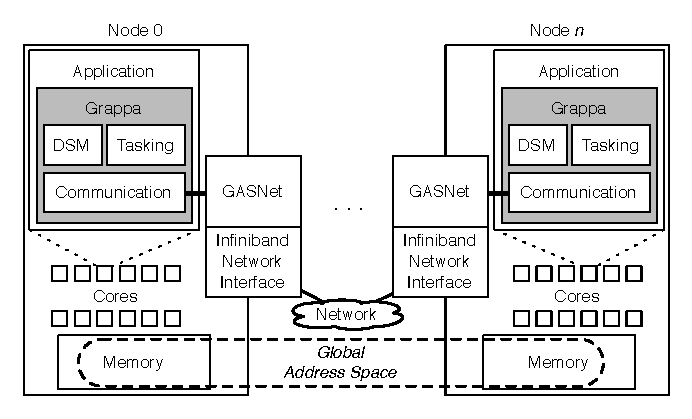
\includegraphics[width=0.95\columnwidth]{figs/system-overview}
\begin{minipage}{0.95\columnwidth}
  \caption{\label{fig:grappa} \Grappa system overview}
\end{minipage}
\vspace{-3ex}
\end{center}
\end{figure}

\begin{description}

\item [Tasking system.] The tasking system supports lightweight multithreading
to tolerate communication latency and global distributed work-stealing (i.e.,
tasks can be stolen from any node in the system), which provides automated
load balancing. The scheduler oversubscribes to have more worker threads than
required for latency tolerance. By having at least four workers per processor
core ready to run at all times, the scheduler can prefetch a worker's state
into cache to lower the likelihood of costly main memory accesses during a
context switch.

\item[Distributed shared memory.] The DSM system provides fine-grain access to
data anywhere in the system. It supports normal access operations such as
\emph{read\/} and \emph{write\/} as well as synchronizing operations such as
\emph{fetch-and-add\/}~\cite{fetchandadd}. It also offers explicit local
caching of any memory in the system, and delegates that directly operate on
remote data. The memory model offered is similar to what underpins
C/C++~\cite{N2480,N2800}, so it is familiar to programmers. The DSM system
design relies on the lightweight tasking system and communication layer in
order to offer high aggregate random access bandwidth for accessing remote
data.

\item[Communication layer.] The main goal of our communication layer is to
aggregate small messages into large ones.  This process is invisible to the application
programmer. Its interface is based on active messages~\cite{vonEicken92}.
Since aggregation and deaggregation of messages needs to be very efficient, we perform the process in parallel and carefully use lock-free synchronization
operations.

\end{description}


\section{Tasking System}

Below we discuss the implementation of our task management support and then
describe how applications expose parallelism to the \Grappa runtime.

\subsection{Task Support Implementation}

The basic unit of execution in \Grappa is a {\em task}. Each hardware core has
a single operating system thread pinned to it. When tasks are ready to
execute, they are mapped to a {\em worker}, which is akin to a user-level
thread. % \Grappa keeps a large pool of workers per hardware core.

\paragraph{Tasks} 
Tasks are specified with a ``functor'' object that holds both code to execute and initial state. The functor can be specified with a function pointer and explicit arguments, a C++ struct that overloads the parentheses operator, or a C++11 lambda. These objects, typically very small (on the order of 64 bytes), hold read-only values such as an iteration index and pointers to common data or synchronization objects. These task functors can be serialized and transported around the system, and eventually executed by a worker, as described next.

\paragraph{Workers} Workers execute application and system (e.g.,
communication) tasks. A worker is simply a collection of status bits and a
stack, allocated at a particular core. When a task is ready to be executed it
is assigned to a worker, which executes the task functor on its own stack. 
Once a task is mapped to a worker it stays with that worker until it finishes.

\paragraph{Scheduling} During execution, a worker yields control of its core
whenever it performs a long-latency operation, allowing the processor to
remain busy while waiting for the operation to complete. In addition, a
programmer can direct scheduling explicitly via the \Grappa API calls shown in
Figure~\ref{fig:scheduling}. To minimize yield overhead, the \Grappa scheduler
operates entirely in user-space and does little more than store state of one
worker and load that of another.

\begin{figure}[htbp]
  \begin{center}
	\begin{tabular}{l}
    \texttt{\scriptsize yield() } \\
      Yields core to scheduler, enqueuing caller to be \\ scheduled again soon \\
    \texttt{\scriptsize suspend() }  \\
      Yields core to scheduler, enqueuing caller only once \\ another task calls wake \\
    \texttt{\scriptsize wake( task * $t$ ) } \\
      Enqueues some other task $t$ to be scheduled again soon \\
	\end{tabular}
    \begin{minipage}{0.95\columnwidth}
      \caption{\label{fig:scheduling} \Grappa scheduling API } 
    \end{minipage}
  \end{center}
\end{figure}

Each core in a \Grappa system has its own independent scheduler. The scheduler
has a single FIFO queue of active \emph{workers} ready to execute, the {\it
ready worker queue}. Each scheduler also has three queues of \emph{tasks}
waiting to be assigned a worker:

\begin{itemize}

\item {\it deadline task queue}, a priority queue of tasks that are executed according to task-specific deadline constraints;

\item {\it private task queue}, a FIFO queue of tasks that must run on
this core and therefore is not subject to stealing;

\item {\it public task queue},  a LIFO queue of tasks that are
  waiting to be matched with workers. It is a local partition of a shared
  task pool.

\end{itemize}


Whenever a task yields or suspends, the scheduler makes a decision about what
to do next. First, any task in the deadline task queue who's deadline
constraint is met is chosen for execution. This queue manages high priority
system tasks, such as periodically servicing communication requests. Second,
the scheduler determines if any workers with running tasks are ready to
execute; if so, one is scheduled. Finally, if there are no workers ready to
run, but there are tasks waiting to be matched with workers, an idle worker is
woken (or a new worker is spawned), matched with a task, and scheduled.

\paragraph{Context switching} 
\Grappa context switches between workers non-preemptively. As with other
cooperative multithreading systems, we treat context switches as function
calls, saving and restoring only the callee-saved state as specified in the
x86-64 ABI~\cite{amd64:abi:2012}. This involves saving six general-purpose
64-bit registers and the stack pointer, as well as the 16-bit x87 floating
point control word and the SSE context/status register. Thus, the minimum
amount of state a cooperative context switch routine must save, according to
the ABI, is 62~bytes.

Since \Grappa keeps a very large number of active workers, their context data
will not fit in cache. Therefore, the scheduler has to perform very careful
prefetching in order to reduce context switch cost to a minimum. We determined
empirically that prefetching the fourth worker in the scheduling order is
sufficient. We also prefetch three cache lines from the stack for each worker.
This makes context switching effectively free of cache misses even to hundreds
of thousands of threads. We provide an analysis of our context switch
performance in Section~\ref{eval:basic}.

\paragraph{Work stealing} 
When the scheduler finds no work to assign to its workers, it commences to
steal tasks from other cores using an asynchronous \texttt{call\_on} active
message. It chooses a victim at random until it finds one with a non-zero
amount of work in its public task queue. The scheduler steals half of the
tasks it finds at the victim. Work stealing is particularly interesting in
\Grappa since performance depends on having many active worker threads on each
core. Even if there are many active threads, if they are all suspended on
long-latency operations, then the core is underutilized.

\subsection{Expressing Parallelism}

\Grappa programmers focus on expressing as much parallelism as possible
without concern for where it will execute. \Grappa then chooses where and when
to exploit this parallelism, scheduling as much work as is necessary on each
core to keep it busy in the presence of system latencies and task dependences.

\Grappa provides four methods for expressing parallelism, shown in
Figure~\ref{fig:expressing-parallelism}. First, when the programmer identifies
work that can be done in parallel, the work may be wrapped up in a function
and queued with its arguments for later execution using a \texttt{spawn}.
Second,
the programmer can invoke a parallel for loop with \texttt{parallel\_for}, provided that the trip count is
known at loop entry. The programmer specifies a function pointer along with
start and end indices and an optional threshold to control parallel overhead.
\Grappa does {\em recursive decomposition} of iterations, similar to Cilk's
cilk\_for construct~\cite {cilkforimplementation}, and TBB's {\tt
parallel\_for}~\cite{intel_tbb}. It generates a logarithmically-deep tree of
tasks, stopping to execute the loop body when the number of iterations is
below the required threshold. Third, a programmer may want to execute an active message; that is, to run a
small piece of code on a particular core in the system without waiting for
execution resources to be available. Custom synchronization primitives, for example, execute this way as a function executed on the core where the data
lives. \Grappa provides the \texttt{call\_on} call for this purpose.

\begin{figure}[htbp]
  \begin{center}
	\begin{tabular}{l}
    \texttt{\scriptsize spawn( Functor f )} \\
      Creates a new stealable task \\
    \texttt{\scriptsize parallel\_for( start, end, Functor iteration )} \\
      Executes iterations of a loop as stealable tasks that \\
      take the iteration index as an argument  \\
    \texttt{\scriptsize call\_on( core, Functor f )} \\ 
      Runs a limited function on a specific core without \\
      consuming \Grappa execution resources 
	\end{tabular}
    \begin{minipage}{0.95\columnwidth}
      \caption{\label{fig:expressing-parallelism} \Grappa API: expressing parallelism
      } % \vspace{-4ex}}
    \end{minipage}
    %\vspace{-3ex}
  \end{center}
\end{figure}

Figure~\ref{fig:sample} shows sample code using \Grappa for a parallel tree
search. The important aspect to note is that the code looks very similar to
what would be written for single shared-memory system, without any concern about data locality or communication.

\begin{figure}[htbp]
\begin{center}
\begin{scriptsize}
\begin{verbatim}
class node_t {
  key_t   key
  int64_t numChildren;
  GlobalAddress<node_t *> children;
};

void search(GlobalAddress<node_t *> node, key_t key) {
  if (node->key == key) {
    result = node;
    return;
  }
  parallel_for(0, node->numChildren, [=](int index) {
    spawnTask([=]{
      search(node->children[index], key);
    });
  });
}
\end{verbatim}
\end{scriptsize}

    \begin{minipage}{0.95\columnwidth}
      \caption{\label{fig:sample} Sample \Grappa code illustrating a parallel tree search similar to the unbalanced tree search benchmark we describe later.}
    \end{minipage}

\end{center}
\end{figure}



\section{Distributed Shared Memory}
\label{sec:memory}

Applications written for \Grappa utilize two forms of memory: local and
global. Local memory is local to a single core within a node in the system.
Accesses occur through conventional pointers. Applications use local accesses for a
number of things in \Grappa: the stack associated with a task, accesses to
localized global memory in caches (see below), and accesses to debugging
infrastructure local to each system node. Local pointers cannot access
memory on other cores, and are valid only on their home core.

Large data that is expected to be shared and accessed with low locality is
stored in \Grappa's global memory. All global data must be accessed through
calls into \Grappa's API, shown in Figure~\ref{fig:accessing-memory}. 

\TODO{worth mentioning localized access for data-parallel stuff, along
    with reasoning about local vs remote accesses as in the PGAS world}

\paragraph{Global memory addressing} \Grappa provides two methods for storing
data in the global memory. The first is a distributed heap striped across all
the machines in the system in a block-cyclic fashion. The
\texttt{global\_malloc} and \texttt{global\_free} calls are used to allocate
and deallocate memory in the global heap. Addresses to memory in the global
heap use \emph{linear addresses}. Choosing the block size involves trading off
sequential bandwidth against aggregate random access bandwidth. Smaller block
sizes help spread data across all the memory controllers in the cluster, but
larger block sizes allow the locality-optimized memory controllers to provide
increased sequential bandwidth. The block size, which is configurable, is
typically set to 64 bytes, or the size of a single hardware cache line, in
order to exploit spatial locality when available.

\Grappa also allows any local data on a core's stacks or heap to be exported
to the global address space to be made accessible to other cores across the
system. Addresses to global memory allocated in this way use \emph{2D global
addresses}. This uses a traditional PGAS (partitioned global address
space~\cite{upc:2005}) addressing model, where each address is a tuple of a
rank in the job (or global process ID) and an address in that process. The
lower 48 bits of the address hold a virtual address in the process. The top
bit is set to indicate that the reference is a 2D address (as opposed to
linear address). This leaves 15~bits for network endpoint ID, which limits our
scalability to $2^{15}$ cores. Any node-local data can be made accessible
to other cores in the system by wrapping the address and node ID into a 2D
global address. This address can then be accessed with a delegate operation
and even be buffered by other cores. The address is converted at the destination
into a canonical x86 address by replacing the upper bits with the
sign-extended upper bit of the virtual address. 2D addresses may refer to
memory allocated from a single processes' heap or from a task's stack.
Figure~\ref{fig:memory-structure} shows how 2D and linear addresses can refer
to other cores' memory.


\begin{figure}[htbp]
  \begin{center}
    \begin{minipage}{0.95\columnwidth}
	\small
  \begin{description}
    \item[Allocation in the global heap:] \hfill \\
      	\lstinline[style=grappa]{GlobalAddress<T> global_malloc<T>( size )} \hfill \\
      	\lstinline[style=grappa]{global_free( GlobalAddress<T> )}  \hfill
    \item[Delegate operations:] \hfill \\
      	\lstinline|T    delegate_read( GlobalAddress<T>)|  \hfill \\
      	\lstinline|Promise<T> delegate_read_async( GlobalAddress<T> )|  \hfill \\
      	\lstinline|void delegate_write( GlobalAddress<T>, T value)| \hfill \\
      	\lstinline|void delegate_write_async( GlobalAddress<T>, T value)| \hfill \\
      	\lstinline|bool delegate_cas( GlobalAddress<T>, T cmp, T set)| \hfill \\
      	\lstinline|T    delegate_fetch_inc( GlobalAddress<T>, T inc)| \hfill \\
      	\lstinline|void delegate_inc_async( GlobalAddress<T>, T inc)|  \hfill\\ 
%        \lstinline|void buffer_acquire( GlobalAddress<T>, local_buf, {RO,RW,WO})| \hfill \\
%        \lstinline|void buffer_release( GlobalAddress<T>, local_buf )| \hfill
    % Perform buffer operations to acquire/release global data.
    % Acquire copies all data to local node and returns a pointer.
    % For write acquire, release copies data back to global memory.
	\end{description}
      \caption{\label{fig:accessing-memory} \Grappa API for memory accesses.}     \end{minipage}
  \end{center}
\end{figure}

\begin{figure}[t]
\begin{center}
  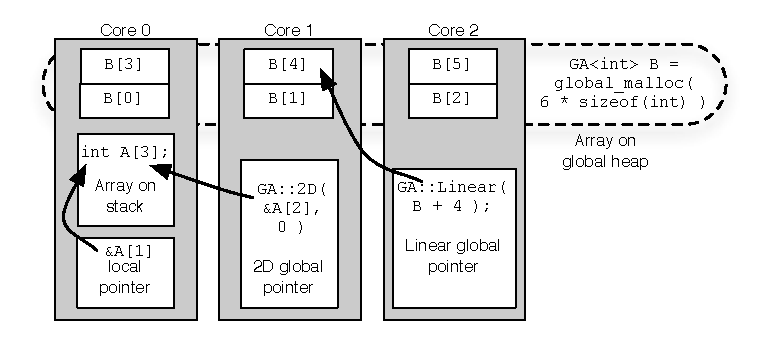
\includegraphics[width=0.95\columnwidth]{figs/memory-structure}
\begin{minipage}{0.95\columnwidth}
  \caption{\label{fig:memory-structure} Global memory referencing in \Grappa}
\end{minipage}
\vspace{-3ex}
\end{center}
\end{figure}

\paragraph{Global memory access} 
Access to \Grappa's distributed shared memory is provided through  {\em
delegate\/} operations, which are short memory accesses performed at the memory
location's home node. When the data access pattern has
low-locality, it is more efficient to modify the data on its home core rather
than bringing a copy to the requesting core and returning it after
modification. Delegate operations~\cite{Nelson:hotpar11, delegated:oopsla11}
provide this capability. Applications can dispatch computation to be performed
on individual machine-word sized chunks of global memory to the memory system
itself.
Delegates can execute arbitrary code, provided they do not block, to ensure communicator workers make progress. Provided they touch only memory owned by a single core, we can use them to perform simple
\emph{read\/}/\emph{write\/} operations to global memory, as well as more complex \emph{read-modify-write\/} operations (e.g., \emph{fetch-and-add\/}). We use these primitive operations to implement higher-level synchronization mechanisms such as mutexes, condition variables, and full-empty bits.

Delegate operations are \emph{always\/} executed at the home core of their
address. The remote operation may not perform any operations that could cause
a context switch; this ensures any modifications are atomic. We limit delegate
operations to operate on objects in the 2D address space or objects that fit
in a single block of the linear address space so they can be satisfied with a
single network request. Given these restrictions, we can ensure that delegate
operations for the same address from multiple requesters are always serialized
through a single core in the system, providing atomic semantics without using
actual atomic operations (and thus avoiding their typical high cost).

Delegate operations can be either {\em blocking\/} or {\em asynchronous}.
With blocking operations, the task issuing the delegate call blocks until
the delegate operation completes, which is necessary, for example, to ensure
that synchronization has finished before continuing. On the other hand, remote data
accesses often can overlap, and delegates with no return value may not need to block the caller. 
To avoid unnecessary waiting, we support asynchronous delegate operations. For reads,
we support a ``futures''-like mechanism which allows tasks to issue reads in parallel and block on the ``promises'' returned. Delegate write operations may also be performed asynchronously, but synchronization is still needed to ensure that asynchronous operations have completed.
\Grappa provides a \texttt{GlobalCompletionEvent} synchronization object, which asyncronous operations (including tasks) can be enrolled. Tasks can block on these objects to be woken when all enrolled operations are complete.
% \TODO{augment this with our bulk futures ie global completions}

When programmers want to operate on data structures spread across
multiple nodes, accesses must be expressed as multiple delegate
operations along with with appropriate synchronization
operations. \Grappa's API also includes calls for gathering and scattering
contiguous blocks in the global heap, but the user is responsible for
ensuring correct synchronization.

\paragraph{Memory consistency model discussion} As mentioned earlier, all
synchronization operations are done via delegate operations. Since they all
execute on their home core in some serial order, they are guaranteed to be globally linearizable~\cite{herlihy1990linearizability}, with their
updates visible to all cores across the system in the same order. In addition, only one synchronous delegate will be in flight at a time from a particular task. Therefore, synchronization operations from a particular task are not subject to reordering. 
% \TODO{I think we can support multiple delegates in parallel from a task as
% long as we block on them before counting on them being complete. see my
% description above about the \emph{future/promise} delegates we have now. Not
% sure if there's a strong example of when this is useful for synchronization
% (though it's definitely useful for reads/writes), acquiring multiple locks
% doesn't work because we have to acquire locks in order to prevent deadlock.}
Consequently, all synchronization operations execute in program order and are
made visible in the same order to all cores in the system. These properties
are sufficient to guarantee a memory model that offers sequential consistency
for data-race-free programs~\cite{AdveHill1990} (all accesses to shared data
are separated by synchronization). This is the memory model that underpins
C/C++~\cite{N2480,N2800}.

Note, however, that if the application code uses explicit buffers or
asynchronous delegates to access shared data, all updates must be published back to
the home core before the synchronization operation that protects the data is
performed. This is done using release operations on cached regions and using
the \texttt{GlobalCompletionEvent} object to determine that asynchronous
delegates have completed.



\TODO{admit the lack of a synchronization feature for lightweight
    transactions across two or more domains. Talk about using the same
    philosophy of moving data along with the sync (same as a real
    cache) and utilizing latency tolerance. Then say further is out of
    scope for this paper.}



\section{Communication Support}
\label{sec:communication}

\Grappa's communication support has two layers: user-level messaging interface
based on active messages; and network-level transport that supports request
aggregation for better communication bandwidth.

\paragraph{Active messages interface} At the upper (user-level) layer, \Grappa
implements asynchronous active messages~\cite{vonEicken92}. Each message
consists of a function pointer, an optional argument payload, and an optional
data payload. 

\paragraph{Message aggregation} In our experiments the vast majority of upper
layer message requests are smaller than 44~bytes. Our measurements confirm
manufacturers' published data [15]; with 44-byte packets, the available
bisection bandwidth is only a small fraction (3\%) of the peak bisection
bandwidth. As mentioned earlier, commodity networks including InfiniBand
achieves their peak bisection bandwidth only when the packet sizes are
relatively large -- on the order of multiple kilobytes. The reason for this
discrepancy is the combination of overheads associated with handling each
packet (in terms of bytes that form the actual packet, processing time at the
card, multiple round-trips on the PCI Express bus and processing on the CPU
within the driver stack). Consequently, to make the best use of the network,
we must convert small messages into large ones.

\paragraph{Message processing mechanics} Since communication is very frequent
in \Grappa, aggregating and sending messages efficiently is very important. To
achieve that, \Grappa makes careful use of caches, prefetching, and lock-free
synchronization operations.

Each processing core of a system node maintains an array of outgoing
message lists.  The array size is the number of system cores in the
\Grappa system.  The outgoing message lists and messages are located
in a region of memory shared across all cores in a \Grappa node (thus
enabling cores to peek at each other's message lists). When a task
sends a message, it allocates a buffer (typically on its stack),
determines the destination system node, and links the buffer into the
corresponding linked list.

Each processing core in a given system node is responsible for
aggregating and sending the resulting messages from all cores on
that node to a set of destination nodes.  Each core periodically
executes a task responsible for sending messages.  This task examines
the private (to each core) message lists for each destination node it
is responsible for managing and, if the list is long enough or a
message has waited past a time-out period, all messages to a given
destination system node from that source system node are sent.
Aggregating and sending a message involves manipulating a set of
shared data-structures (the message lists). This is done using CAS
(compare-and-swap) operations to avoid high synchronization costs.
Note that we use a per-core array of message lists
that is only periodically modified across processor cores after
experimentally determining that this approach was faster (sometimes
significantly) than a global per-system node array of message lists.

Each node has a region of memory with send buffers where the final aggregated
messages are built. These buffers are visible to the network card, and
messages are sent with user-mode operations only. When the worker
responsible for outbound messages to a given system node has received a
sufficient number of message send requests or a timeout is reached, the
linked list of messages is walked and messages are copied to a send buffer.
This process requires careful prefetching because most of the outbound
messages are \emph{not\/} in the processor cache at this time (recall that a
core can be aggregating messages originating from other cores in the same
node). Once the send buffer has been formed, it is handed off to GASNet for
transfer to the remote system node. RDMA is used if the underlying network
supports it. 

There are two useful consequences of forming the send buffer at the time of
message transmission instead of along the way as individual upper layer
message send requests are received. First, as previously mentioned, most of the
messages are not in the cache and prefetching is used to run ahead in the
linked list of messages in order to avoid cache misses. But once the send
buffer is formed, it is in the cache (for the most part). Hence, when it is
handed off to GASNet for transfer across the physical wire, the network card
can pull the message buffer from the processor cache instead of main memory,
which we have found speeds performance. The second consequence of this
decision is that we do not need to pre-allocate buffers for all destination
nodes in the system, as the buffer can be allocated on the fly. Nevertheless
we have found it efficient to build a flow-control-like protocol of
outstanding message buffers between pairs of system nodes.

Once the remote system node has received the message buffer, a
management task is spawned to manage the unpacking process.  The
management task spawns a task on each core at the receiving
system to simultaneously unpack messages destined for that core.
Upon completion, these unpacking tasks synchronize with the management
task.  Once all cores have processed the message buffer, the management
task sends a reply to the sending system node indicating the
successful delivery of the messages.


%%%% Comments from Jacob. 

% Last paragraph:

% When a buffer is received, all cores deaggregate their messages in parallel.
% This is how it works:
%
%	- the sending core does an RDMA put into a buffer owned by the receiving
%	core. an active message is sent to enqueue this buffer to be processed by a
%	receive worker.
%
%	- the receive worker computes the offsets/lengths of the messages in the
%	buffer for each core on the node. It sends messages through the CAS lists
%	to each core with their offset and length.
%
%	- The cores all deserialize and execute their received active messages.
%	This is done in parallel. Since messages to the same core are stored next
%	to each other in the buffer, this deserialization performs well with the
%	cache and the hardware prefetcher.
%
%  - When the cores are done, they send a message back to the receive worker.
%
%	- Once the receive worker knows all the cores on the node are done with the
%	buffer, it's done. (we then return the buffer pointer to the sending node
%	so it can send again.)
% 
% We should make sure we cite the Threaded Abstract Machine paper too.
% 
% If we haven't already, we should cite Myrinet, U-Net, EMP, and I think
% there's one more. Here are some links:
% 
% http://dl.acm.org/citation.cfm?id=623898&CFID=128100904&CFTOKEN=36373202
% http://dl.acm.org/citation.cfm?id=224061&CFID=128100904&CFTOKEN=36373202
% http://dl.acm.org/citation.cfm?id=582091&CFID=128100904&CFTOKEN=36373202


%\TODO{paper.tex: I know we removed the programming model from the paper and
    % merged into the overview pieces, but I think we need at least a
    % brief summary of the machine model the programmer should be
    % thinking about. 1.large number of tasks, 2.PGAS model for thinking
    % of memory accesses where remote memory is expensive and
    % packets should be large when this is easily expressed, 3.
    % streaming writes are cheaper than writes that require consistency
    % in the task, 4.overlapping read/writes are better than
    % nonoverlapping. Thats a lot to think about but a compiler can at
    % least help with part of 2 and 4 and \Grappa lets you work less
    % hard on 2 by providing aggregation. -BM}

\section{Methodology} \label{sec:method}

To explore the performance of the Grappa runtime we have implemented three algorithms: breadth first search, betweenness centrality, and unbalanced tree search.  These algorithms were implemented for the Cray XMT (our baseline) and for Grappa.  Performance results for Grappa were obtained on a 144 node cluster.  Individual nodes of this cluster contain the hardware depicted in Table~\ref{table:grappanode}.  Nodes are interconnected with both 10G ethernet and infiniband.  For all but startup and configuration, they are configured to communicate over the infiniband network for these experiments.

The metric we use is algorithmic time, which means startup and loading of the data structure (from disk) is not included in the measurement.  Data is collected on real systems, which means minor variations in runtime exist from run to run.  The average of multiple runs are used, and where appropriate, confidence in the result is reported.

One question that must be answered when making a comparison between the
Cray XMT and a typical HPC cluster is what is a fair comparison -- these
systems are quite different.  Three options immediately come to mind:
equal number of processing cores, equal number of network interfaces,
and equal dollars.  We discounted the last option fairly quickly,
because it isn't a lasting data-point -- the cost of hardware shifts
over time, skewing the interpretation of results.  The first option,
cores, has some merit, but Grappa is designed for applications that have
no locality in their computation.  This means almost all of their memory
accesses are remote.  The factor that limits their performance is not
processing, but communicating.  Hence, we have chosen the middle option,
network interfaces as the way to normalize across the XMT and our
cluster.  Each processor in the XMT system has its own network interface
to access shared memory.  In the HPC cluster we use, each processor
(which contains up to 32 cores, although we only use \checkme{6} in our
experiments), has a single infiniband interface.  Hence, for our results
we scale up XMT processors one for one with full system nodes.



\subsection{Systems}

For measurements, we run Grappa on a 144-node cluster of AMD Interlagos
processors. Nodes have 32-core (every pair share a floating-point unit)
2.1-GHz processors, 64GB of memory, and \checkme{a 40Gb Super-terrific
Happy-Lucky} infiniband network card.   The cluster uses a
\checkme{McNugget} infiniband switch. We configure the nodes to have 32
1-GB hugepages to minimize TLB misses for the random access patterns we
expect from irregular applications.\comment{The results we present are for this
machine, but we have also run Grappa on our own 12-node Intel Xeon
Westmere cluster, which performs similarly.}

We compare to the MTA using a 128-node Cray XMT (3rd generation MTA). 
Each node consists of a 500-MHz MTA Threadstorm multithreaded
processor that supports 128 streams. The machine uses Cray's proprietary
SeaStar2 interconnection network.

\subsection{Applications}

We have used three benchmarks to explore the performance of Grappa:

\comment{
    Traversal of an unbalanced, unpartitioned tree captures the foundations for implementing most forms of irregular parallelism. 
Recursion is found in every irregular divide and conquer algorithm.
Loops, even regular ones, must be dynamically scheduled to get good
load balance when run on a large, non-uniform system. Nested
parallelism involves fine-grain creation of dynamic amounts of work.
Dataflow..
}

\paragraph{Unbalanced tree search in-memory (UTS-Mem)} Unbalanced Tree
Search (UTS) is a benchmark for evaluating the programmability and
performance of systems for parallel applications that require dynamic
load balancing \cite{Olivier:uts2006}. It involves traversing an
unbalanced implicit tree: at each vertex, its number of children is
sampled from some probability distribution, and this number of new nodes
are added to a work queue to be visited. While this benchmark captures
irregular, dynamic \emph{computation}, we actually want to evaluate
performance of algorithms with irregular \emph{memory} access patterns. 
Thus we augment UTS by using the existing traversal code to create a
large tree in memory, and then we traverse the in-memory tree. We call
this benchmark UTS-Mem, and the timed portion is this traversal of the
in-memory tree. This in-memory traversal has no knowledgeable of the
tree structure beforehand.

%todo: say tree explore is same as a search except we are additionally needing to synchronize on all vertices visited

The Grappa version of the in-memory tree search uses the
asynchronous parallel for loop over a visited vertex's children 
list.  \comment{WTF? -M
A larger threshold can be set to take advantage of this 
locality by processing more child pointers sequentially in a single task.}

\comment{The Grappa version of tree search UTS-mem

\lstset{language=C++,
       basicstyle=\footnotesize,
       tabsize=2}
\begin{lstlisting}
// base of shared vertex_t[]
GlobalAddress<vertex_t> Vertices;        

// base of shared int64_t[]
GlobalAddress<int64_t> ChildrenPointers;  

void search_vertex( id ) {
  GlobalAddress<vertex_t> v_addr = Vertices + id;
  Incoherent<vertex_t>::RO v( v_add, 1 );

  // start index of my children pointers
  childIndex = v->childIndex;    

  // how many children I have
  numChildren = v->numChildren;  

  // parallel loop over the child list for this vertex
  parallel_for(fn=&search_children, start=childIndex, iters=numChildren);
}

void search_children( start, iters ) {
  // take advantage of spatial locality in the array of children
  GlobalAddress<int64_t> child_base_addr = ChildrenPointers + start;
  Incoherent<int64_t>::RO childIds( child_base_addr, iters );

  // spawn a task to visit each child
  for (i = 0..iters) {
    SoftXMT_publicTask( fn=&search_vertex, id=childIds[i] );
  }
}
\end{lstlisting}
}

\paragraph{Breadth-first-search (BFS)}
This is the primary kernel for the Graph500 benchmark and is what currently determines the ranking of machines on the Graph500 list~\cite{graph500list}. As a whole, the Graph500 benchmark suite is designed to bring the focus of system design on data-intensive workloads, particularly large-scale graph analysis problems, that are important among cybersecurity, informatics, and network understanding workloads. The BFS benchmark builds a search tree containing parent nodes for each traversed vertex during the search.  While this is a relatively simple problem to solve, it exercises the random-access and fine-grained synchronization capabilities of a system as well as being a primitive in many other graph algorithms. Performance is measured in \emph{traversed edges per second} (TEPS), where the number of edges is the edges making up the generated BFS tree. One of the reference implementations of Graph500 BFS is for the XMT; this code fails to scale past 16 XMT processors because it does not expose enough parallelism, so we modified the code to use a recursive loop decomposition similar to Grappa's. We compare this modified version against a straightforward Grappa implementation. We do not employ algorithmic improvements, though there are many \cite{Beamer:Graph500,Yoo:FixedPointGraph500}.

\paragraph{Betweenness Centrality}
An important measure of the importance of particular vertices in a network is betweenness centrality (BC) \cite{freeman1979centrality}. By this measure, the ``importance'' of each vertex is computed by finding the fraction of shortest paths that pass through it, which can optionally be approximated by only computing shortest paths using a subset of the vertices as starting points. BC can be useful for understanding which vertices may have the greatest impact, so in social networks this could be the primary person linking two communities. Because it requires multiple breadth-first traversals across the entire graph and in reverse, on power-law degree graphs, this algorithm exercises random accesses rate, and load balancing. It also requires fine-grained synchronization on updates to vertex centrality values because multiple paths will update the same vertex. BC is a kernel in the DARPA High Performance Computing Systems (HPCS) Scalable Synthetic Compact Applications graph analysis (SSCA\#2) benchmark\cite{ssca2}. Performance for BC is also measured in TEPS, where the number of traversed edges is the total number of edges in the graph multiplied by the number of random starting vertices used in the approximate computation. We use the XMT implementation of BC implemented as part of the GraphCT~\cite{GraphCT} library and a comparable Grappa implementation, both of which use the parallel BC algorithm developed by Bader et al.~\cite{bader:bc}.


\section{Evaluation}
\label{sec:evaluation}

The goal of our evaluation is to show that the core pieces of the \Grappa
runtime system, namely our tasking system and the global memory/communication
layer work as expected and together are able to efficiently run irregular
applications. We evaluate \Grappa in three basic steps:

\begin{itemize}

\item We present results that show that the \Grappa runtime is able to sustain
very high concurrency rates and the communication layer is able to sustain a
very high rate of global memory operations. We also show the performance of a
graph kernel that stresses communication and concurrency together.

\item We show how some popular irregular applications running on \Grappa
compare to the Cray XMT and hand-tuned MPI code.

\item We finish with a characterization of system behavior, including
profiling where execution time goes, how aggregation affects message size and
rates, how global memory and work stealing behaves.

\end{itemize}

\subsection{Basic \Grappa Mechanisms}
\label{eval:basic}

\paragraph{User-level context switching.}

As discussed earlier, fast context switching is at the heart of \Grappa's
latency tolerance abilities. We assess context switch overheads using a simple
microbenchmark that has a configurable number of workers, where each worker 
just increments values in a large array. 

\begin{figure}[ht]
    \begin{center}
      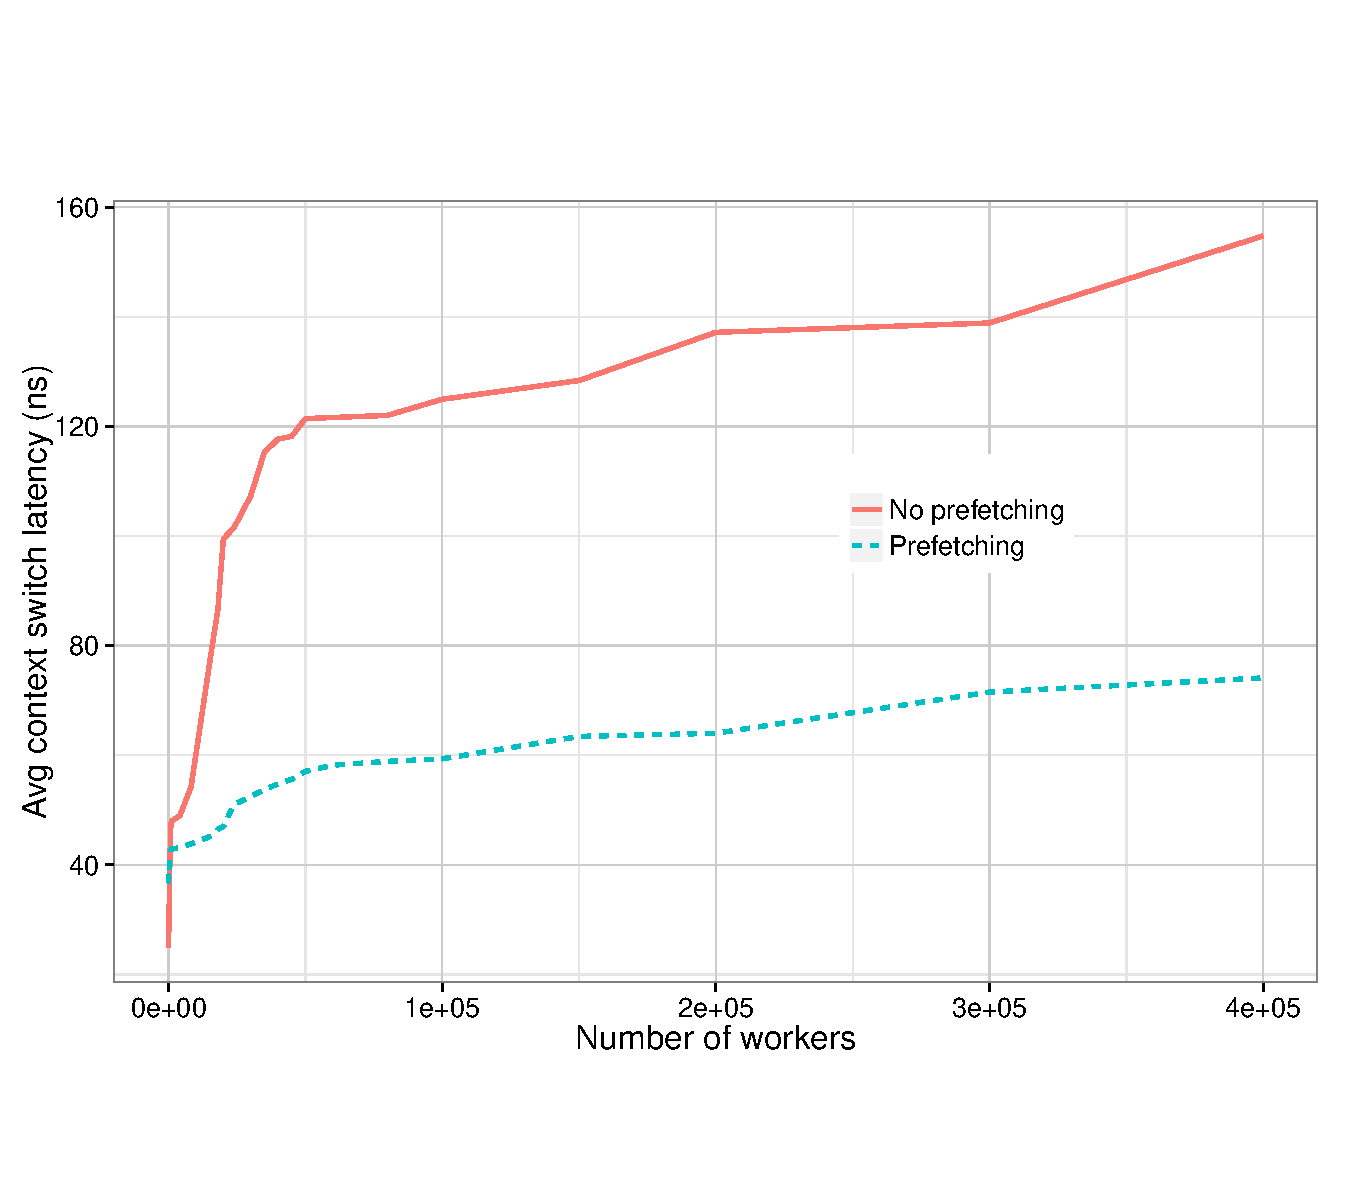
\includegraphics[width=0.5\textwidth]{figs/context_switch_time.pdf}
    \end{center}
    \caption{Average context switch time with and without prefetching.}
    \label{fig:context-switch-exp}
\end{figure}

Figure~\ref{fig:context-switch-exp} shows the average context switch time as
the number of workers grow. There are two important takeaway points from these
data. Context switch time for the number of workers we use ($~$1K workers) is
on the order of 50 ns; and prefetching has significant impact on context
switch time. And context switch time does not grow significantly with the
number of workers --- even with one-half million workers, context switch
is around 75ns.

We also measured (not in the plot) the \emph{rate} of context switch for all
cores in a node, which showed that our rate is limited by off-chip memory
bandwidth. Each context is 4 cache lines (1 for the worker struct and 3 for
stack data), leading to 8 cache line transfers per context switch
(write the previous context, read the next in). The off-chip bandwidth of a
single socket in our system is 270M cache lines per second, which implies that
we can sustain at most 34M context switches per second per socket, which is
almost exactly what we sustain.

In summary, our context switch engine is able to efficiently sustain very high
concurrency and as we will show later, the amount of concurrency sustained is
sufficient the latencies \Grappa needs to hide.

\paragraph{Global memory and communication.} We measure the performance of
\Grappa's global memory and communication layers using a faithful
implementation of the giga updates per second (GUPS) benchmark.
Read-modify-write updates are dispatched at random to a large array. This
benchmark stresses the communication layer of \Grappa separately from the
scheduler, because only a single worker is used per system node.
Figure~\ref{fig:grappa-gups} shows that \Grappa is able to sustain well over a
billion updates per second with 64 nodes. This compares very favorably to
published results~\cite{gups} for other high-end HPC systems.


\begin{figure}[ht]
    \begin{center}
      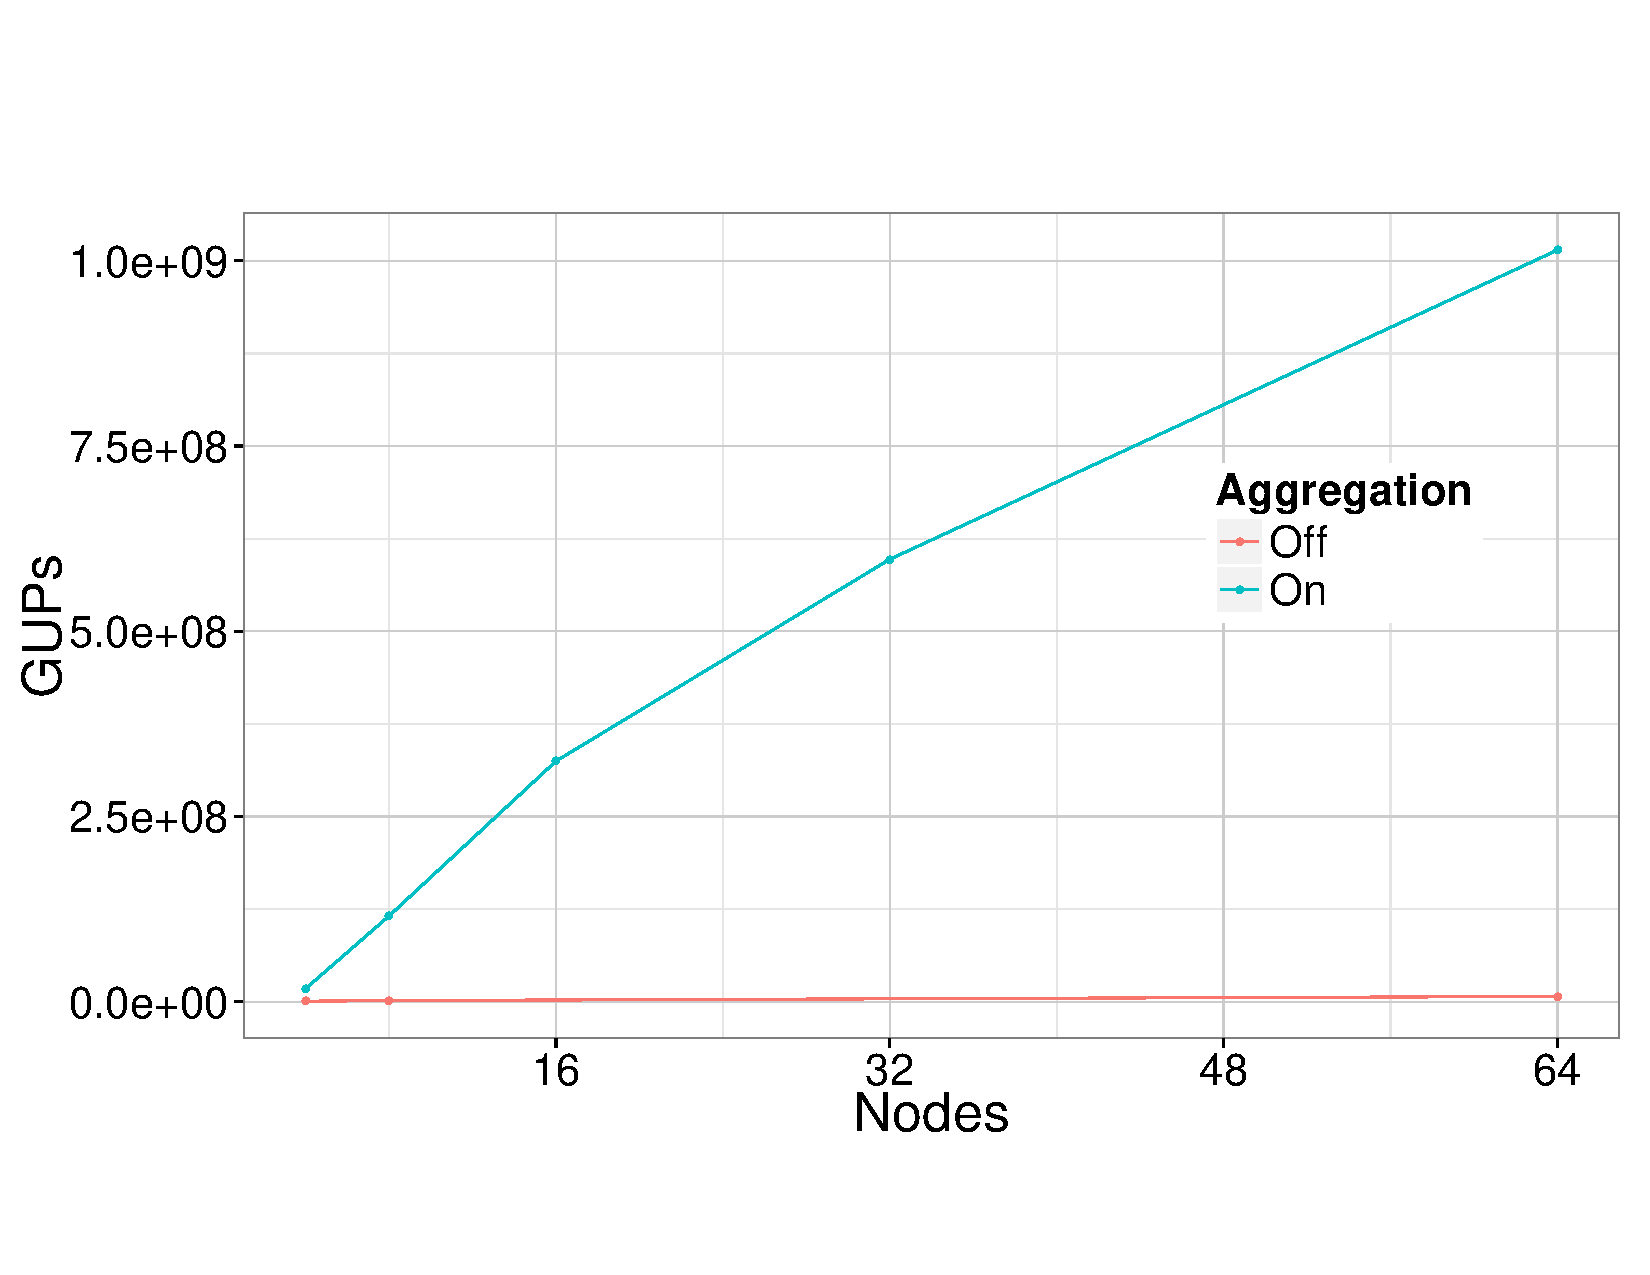
\includegraphics[width=0.5\textwidth]{results/gups/gups.pdf}
    \end{center}
    \caption{GUPS (giga updates per second) for \Grappa as the number of nodes grows.}
    \label{fig:grappa-gups}
\end{figure}

\paragraph{Putting it all together with Unbalanced Tree Search in
    memory (UTS).}
We now show the overall performance of \Grappa running UTS.
Figure~\ref{fig:grappa-uts}. The point of this experiment is to
demonstrate whether \Grappa's context switching and communication layers can in fact
be used together, while balancing workload, to run an irregular application efficiently. 
We look at two classes of trees, T1x and T3x, from the
original benchmark. T1x trees are very shallow and wide, while T3x
trees are very deep. When the access to each vertex is a random
access, the critical path to search T3x trees is very long. On such
trees, we do not expect there to be sufficient concurrency for any
system, including \Grappa, to achieve high throughput. \TODO{plot it
    if time}. To verify this, at the 16-node data point, the average active tasks per
core over the search is 775 and 13 for T1XL and T3L, respectively.

\begin{figure}[ht]
    \begin{center}
      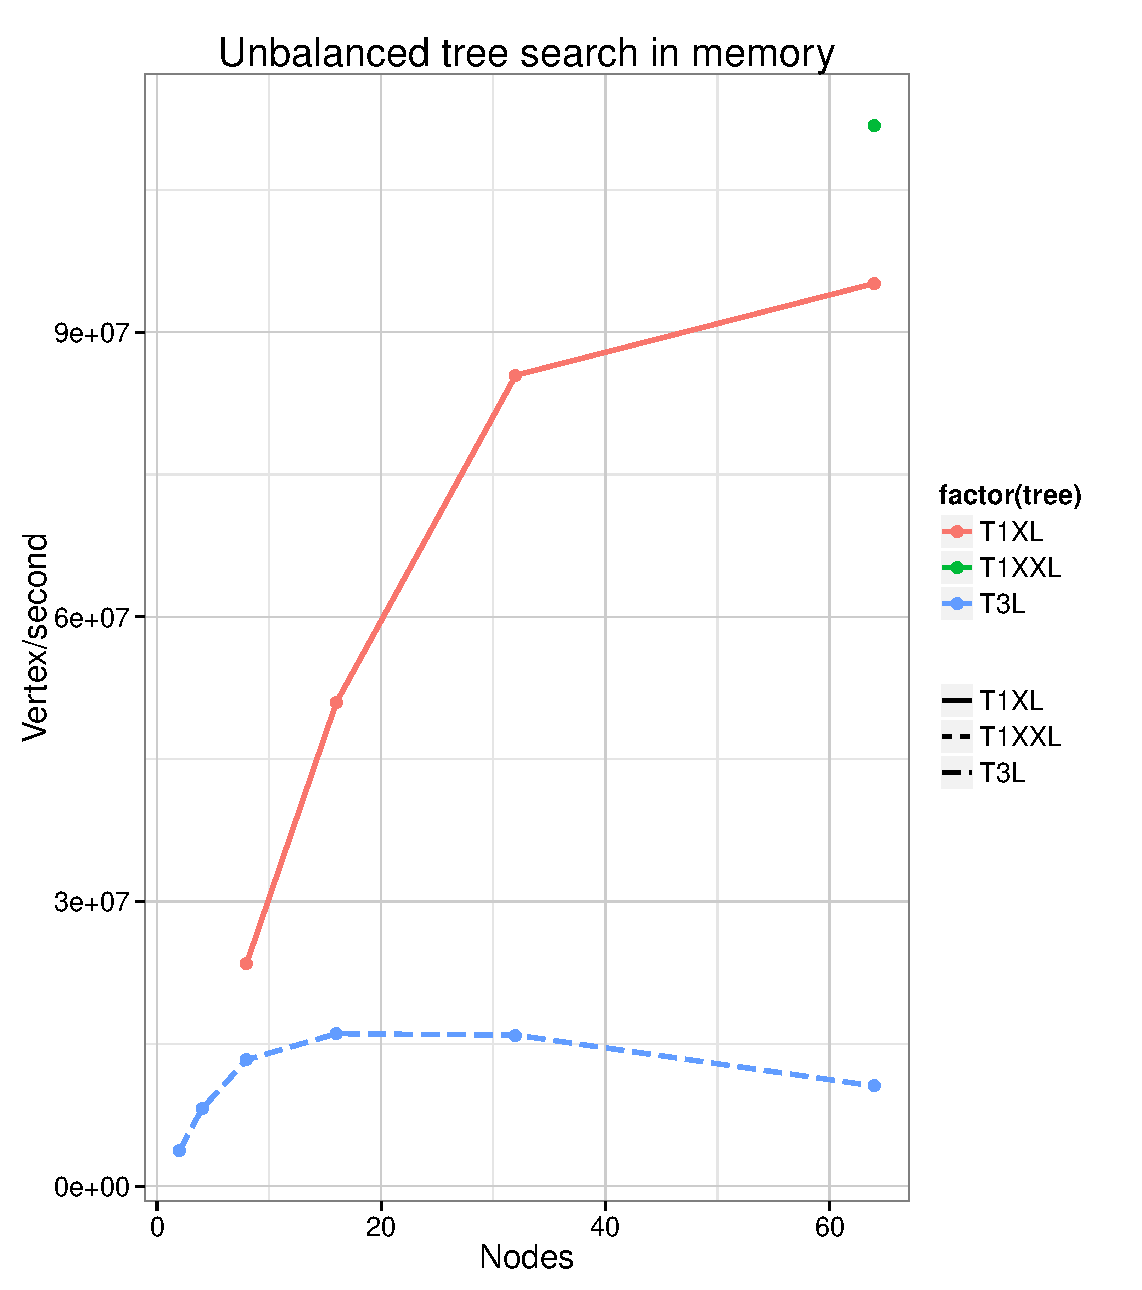
\includegraphics[width=0.5\textwidth]{figs/uts_scale.pdf}
    \end{center}
    \caption{Vertices per second in UTS on \Grappa as the number of nodes grows.}
    \label{fig:grappa-uts}
\end{figure}


\subsection{Comparing \Grappa to Other Systems}

In order to put \Grappa's performance into a general context, we compare it
with XMT running BFS, PageRank, IntSort, GUPS and UTS. Since XMT is a
different hardware platform, we also compare \Grappa with hand-tuned MPI
versions of BFS and GUPS running on the same hardware. Finally, we also
compare it with UTS written for UPC. We run all experiments with 64 nodes.

\begin{figure}[ht]
    \begin{center}
      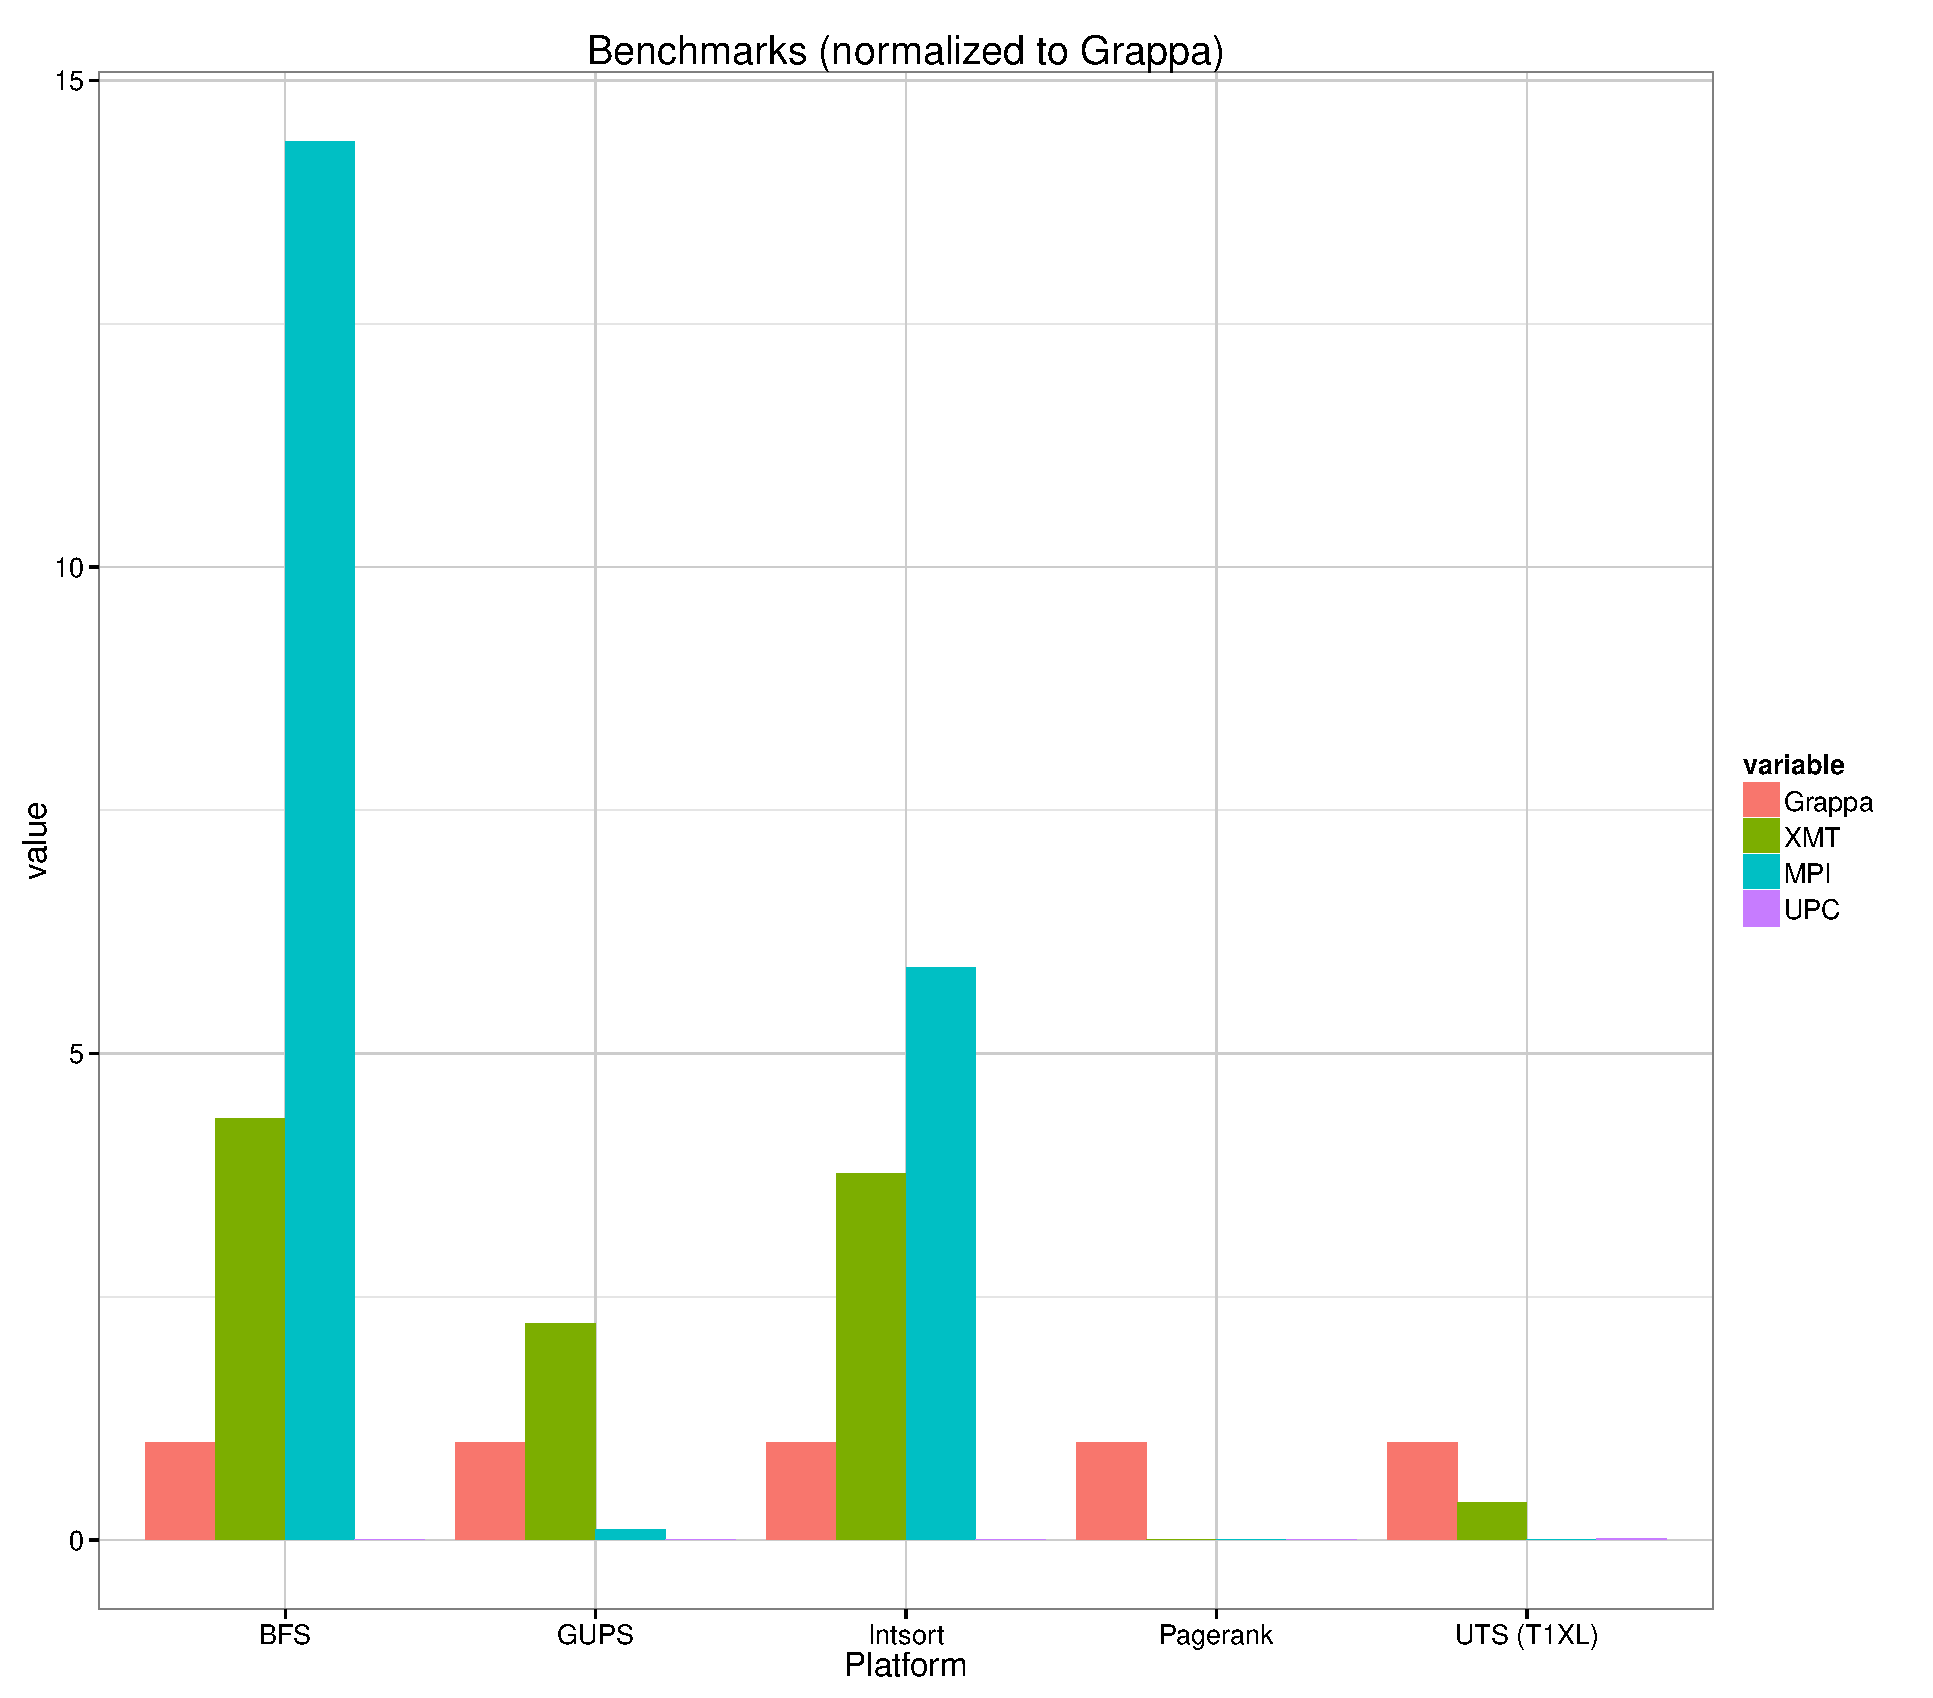
\includegraphics[width=0.5\textwidth]{results/benchmarks.pdf}
    \end{center}
    \caption{Comparing \Grappa with XMT, hand-tuned MPI and UPC.}
%bar chart, one set of bars per benchmark, one bar per system. runtime normalized to grappa.
    \label{fig:grappa-comparisons}
\end{figure}

Figure~\ref{fig:grappa-comparisons} shows the results. Overall, \Grappa is
within striking distance of XMT and UPC performance. However, it underperforms
compared to hand-tuned MPI. Nevertheless, this comparison needs to be taken
with a grain of salt for several reasons. First, we have not spent as much
time tuning \Grappa's implementations. This is supported by inspecting the BFS
MPI implementation we used, which clearly shows that it employs a lot of
algorithmic-specific optimizations. In fact, some of these optimizations
resemble some of what \Grappa does automatically, like message aggregation.
Second, the GUPS results presented earlier suggests that \Grappa performance
can do a lot better. \TODO{update this once we have more results. }

\subsection{Characterization}

\paragraph{Where execution time goes.}


\begin{figure}[ht]
    \begin{center}
      \begin{tabular}{c|c c c c}
        Benchmark     & Comm & User & Idle & Sched \\ \hline
        GUPS          & 6.60  & 42.94   & 47.74 & 2.80 \\
        BFS           & 54.84 & 30.90   & 10.94 & 3.43 \\ 
        Intsort       & 34.28 & 42.00   & 21.31 & 2.47 \\ 
        UTS           & 40.57 & 56.52   &  1.21 & 1.73 \\
        Pagerank      & 76.79 & 20.71   &  0.06 & 2.50 \\
      \end{tabular}
    \end{center}
    \caption{\Grappa\ execution time profile, in percent.}
%bar chart, one set of bars per benchmark, one bar per system. runtime normalized to grappa.
    \label{fig:grappa-profile}
\end{figure}

\TODO{PAGERANK:
    Without parallelizing the dot product, \Grappa cannot achieve
high utilization of workers proportional to the size of the data set.
Also mention that the cost of this is contention at the target
elements of vector.  The other parts of pagerank are super fast
(table?)
}

\paragraph{Message size and latency.}
Distribution if possible. With and without aggregation. 

\begin{figure}[ht]
    \begin{center}
      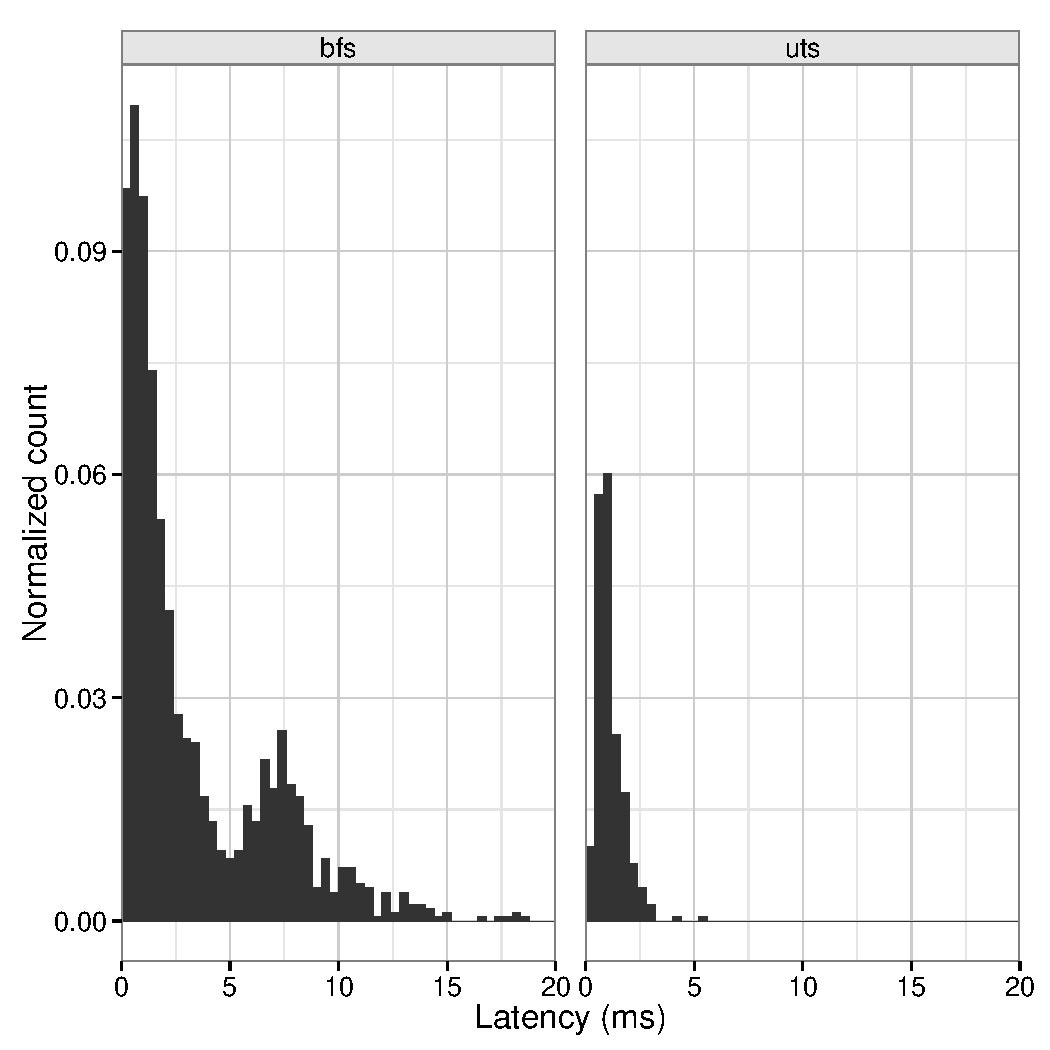
\includegraphics[width=0.5\textwidth]{results/histograms/latency_cmb.pdf}
    \end{center}
    \caption{Round-trip latency of delegate operations.}
%bar chart, one set of bars per benchmark, one bar per system. runtime normalized to grappa.
    \label{fig:grappa-latency}
\end{figure}

\begin{figure}[ht]
    \begin{center}
      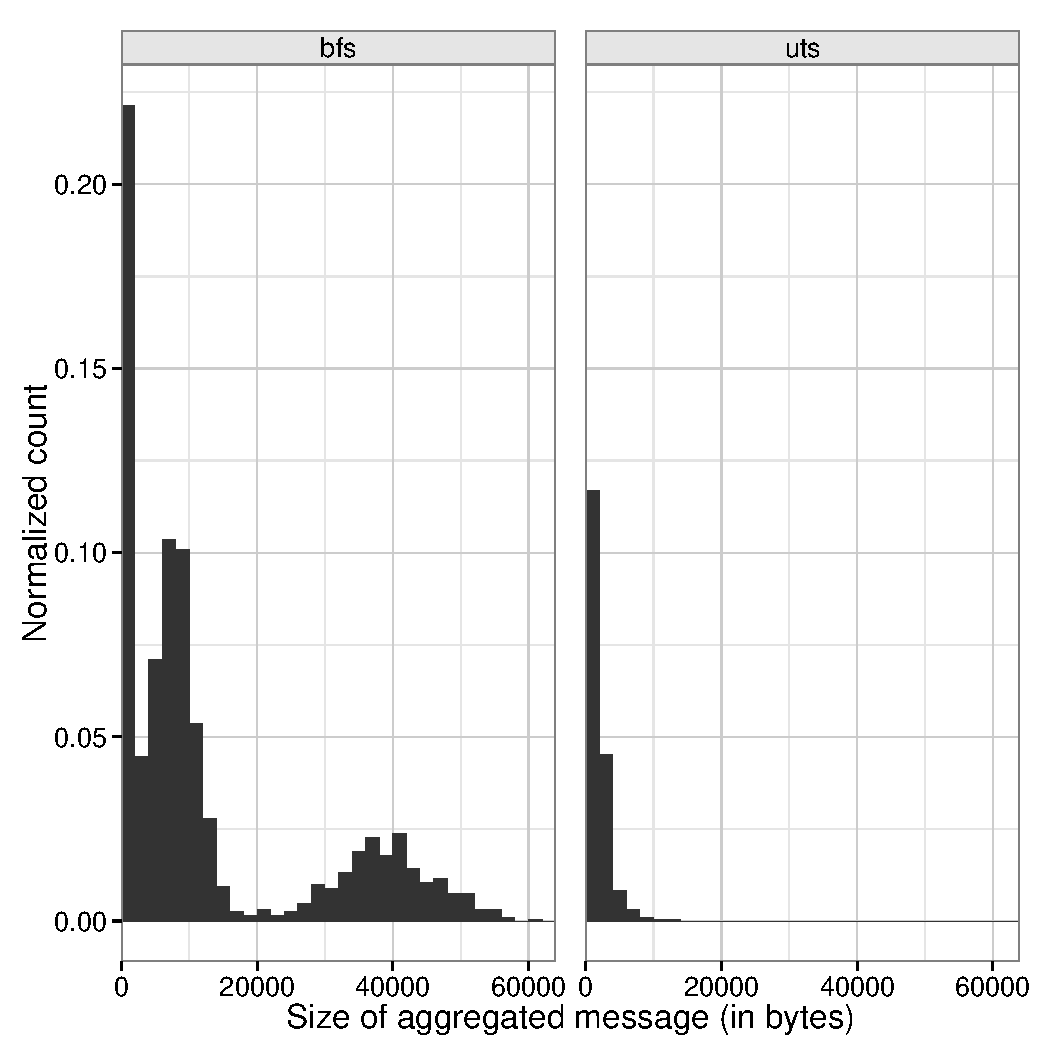
\includegraphics[width=0.5\textwidth]{results/histograms/rdma_bytes_sent_histogram_cmb.pdf}
    \end{center}
    \caption{Distribution of aggregated message sizes.}
%bar chart, one set of bars per benchmark, one bar per system. runtime normalized to grappa.
    \label{fig:grappa-message-size}
\end{figure}


\paragraph{Frequency of remote requests.}

\paragraph{Work stealing behavior.}
Performance loss of not having stealing. Ratio of \# of steals over total \# of task spawns. UTS needs stealing to work. 
















%%%%%%%%%%%%%%%%%%%%%%%%%%%%%%%%%%%%%% OLD %%%%%%%%%%%%%%%%%%

\comment{


Our evaluation begins with presentation of microbenchmark results, establishing
the intrinsic potential of \Grappa to provide random access bandwidth and latency tolerance. 
Next, we present application results, both for \Grappa and for other paradigms, as well
as comparing against the Cray XMT.  Finally, we present the impact of increased aggregation delay
on \Grappa results, thus exploring robustness to network scale.

\subsection{Microbenchmark Results}

\subsubsection{Random Access}
\TODO{Random access feed forward results on \Grappa.  optional: Results we measured for XMT.  Cite MPI results}
\subsubsection{Latency Tolerance}
\TODO{Simple ping test results -- eg, MPI ping, not the full blown aggregation ping test.  Random access blocking results on \Grappa.}
\subsubsection{Scheduling and Robustness}

\begin{figure}[ht]
    \begin{center}
      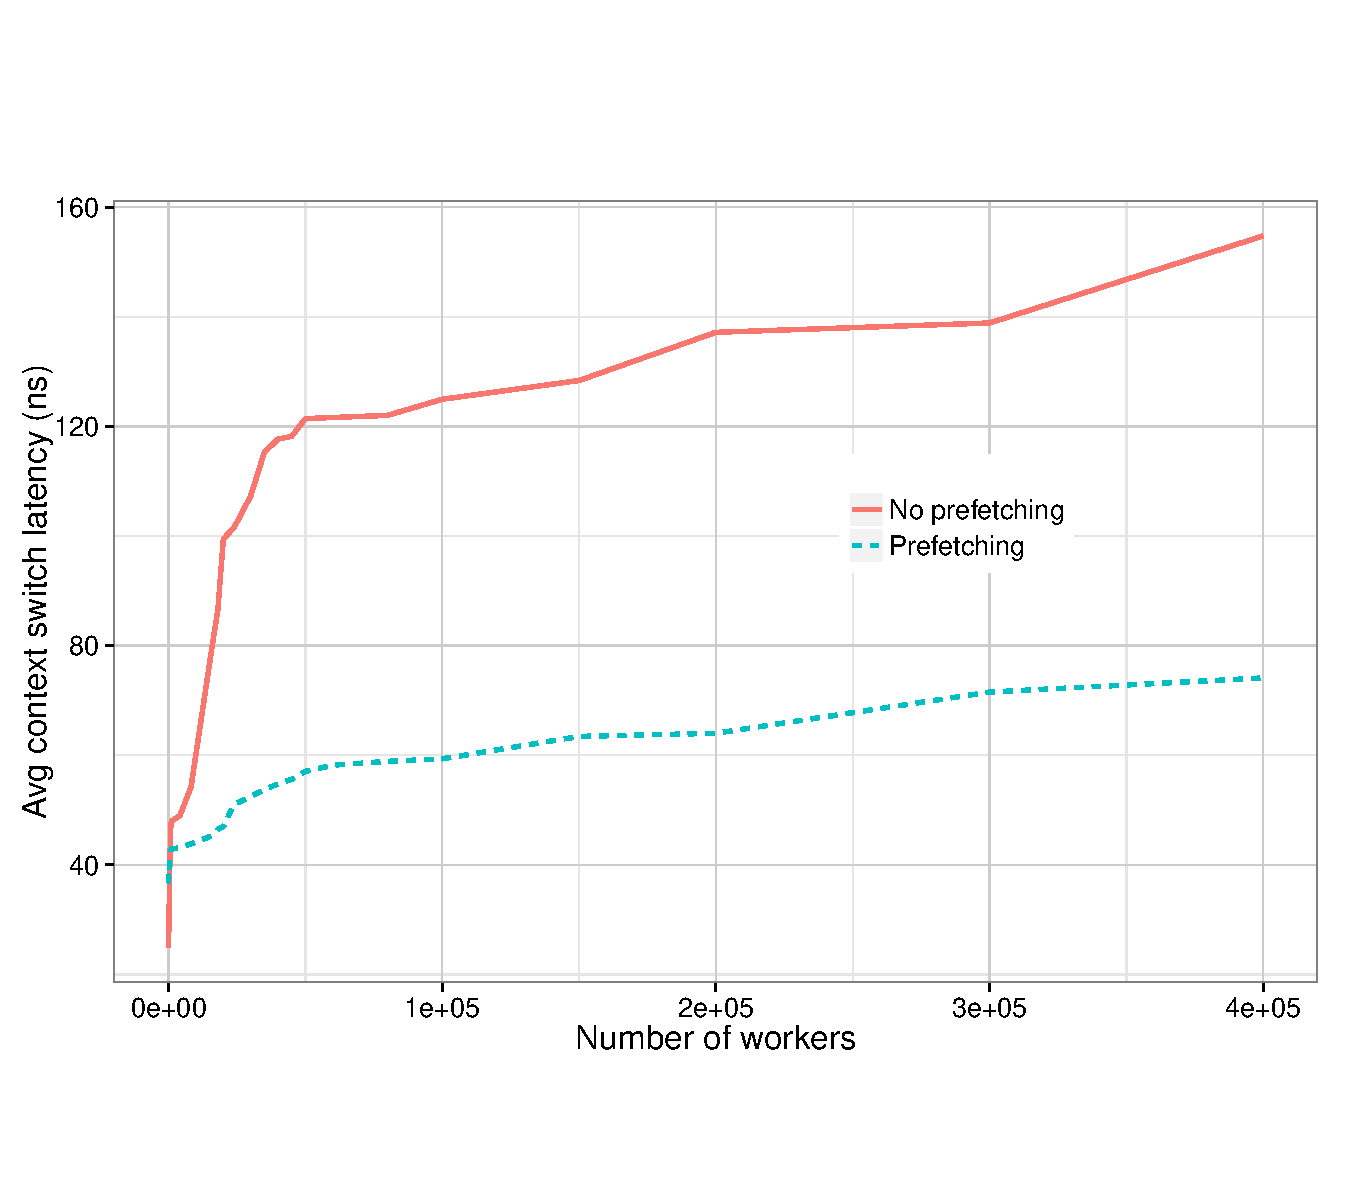
\includegraphics[width=0.5\textwidth]{figs/context_switch_time.pdf}
    \end{center}
    \caption{Average context switch time with 1 and 6 active cores,
        with and without prefetching.}
    \label{fig:context-switch-time}
\end{figure}

\begin{figure}[ht]
    \begin{center}
      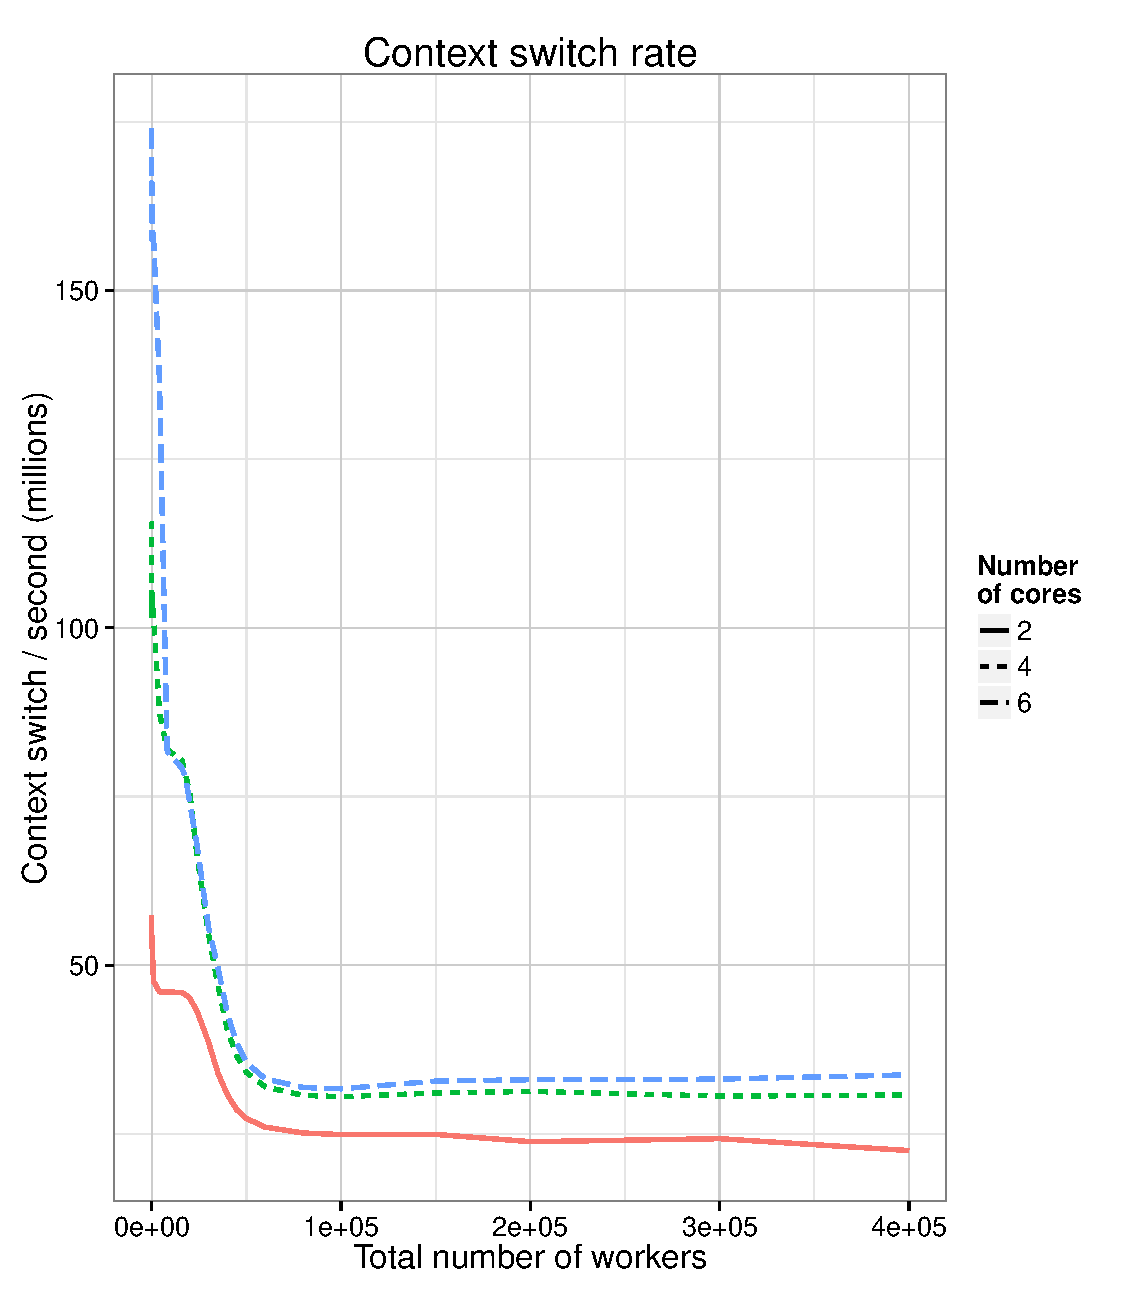
\includegraphics[width=0.5\textwidth]{figs/context_switch_bw.pdf}
    \end{center}
    \caption{Context switch rate with prefetching. Once the total
        size of contexts sufficiently exceeds last-level cache, most
    prefetches go to main memory and the rate becomes limited to the
    off-chip bandwidth.}
    \label{fig:context-switch-time}
\end{figure}

\TODO{Summary of what to write please expand: Reference above plots. Bandwidth of single socket is
    270Mcacheline/s. Each context is 4 cachelines: 1 for worker struct
    and 3 stack cachelines. We must read and write every context, so 8
    cacheline transfers per context switch. This asymptotically
    approaches 33.75Mcontexts/s as you increase the number of contexts
    (fewer and fewer in L3). Note that only 4+ cores reaches full rate
    because these westmere chips are balanced to not achieve full off-chip bandwidth until 4
    cores--bdmyers}

\TODO{Yield test results:  latency \& bandwidth.  Discussion of implications of zillions of contexts on robustness of latency tolerance preshadowing ~\ref{sec:scaling}}

\subsection{Application Results}
To evaluate \Grappa's performance with respect to the XMT, we ran each
of our three benchmarks on up to 16 nodes of each machine. \Grappa used
6 cores per node, with the best parameters chosen for each point. In
some cases, the XMT could not run the benchmark with 2 nodes, so the
point is omitted. \TODO{rewrite this!}
\subsubsection{Unbalanced Tree Search}\TODO{rewrite with new results}
%% UTS: performance comparison
\begin{figure}[ht]
    \begin{center}
      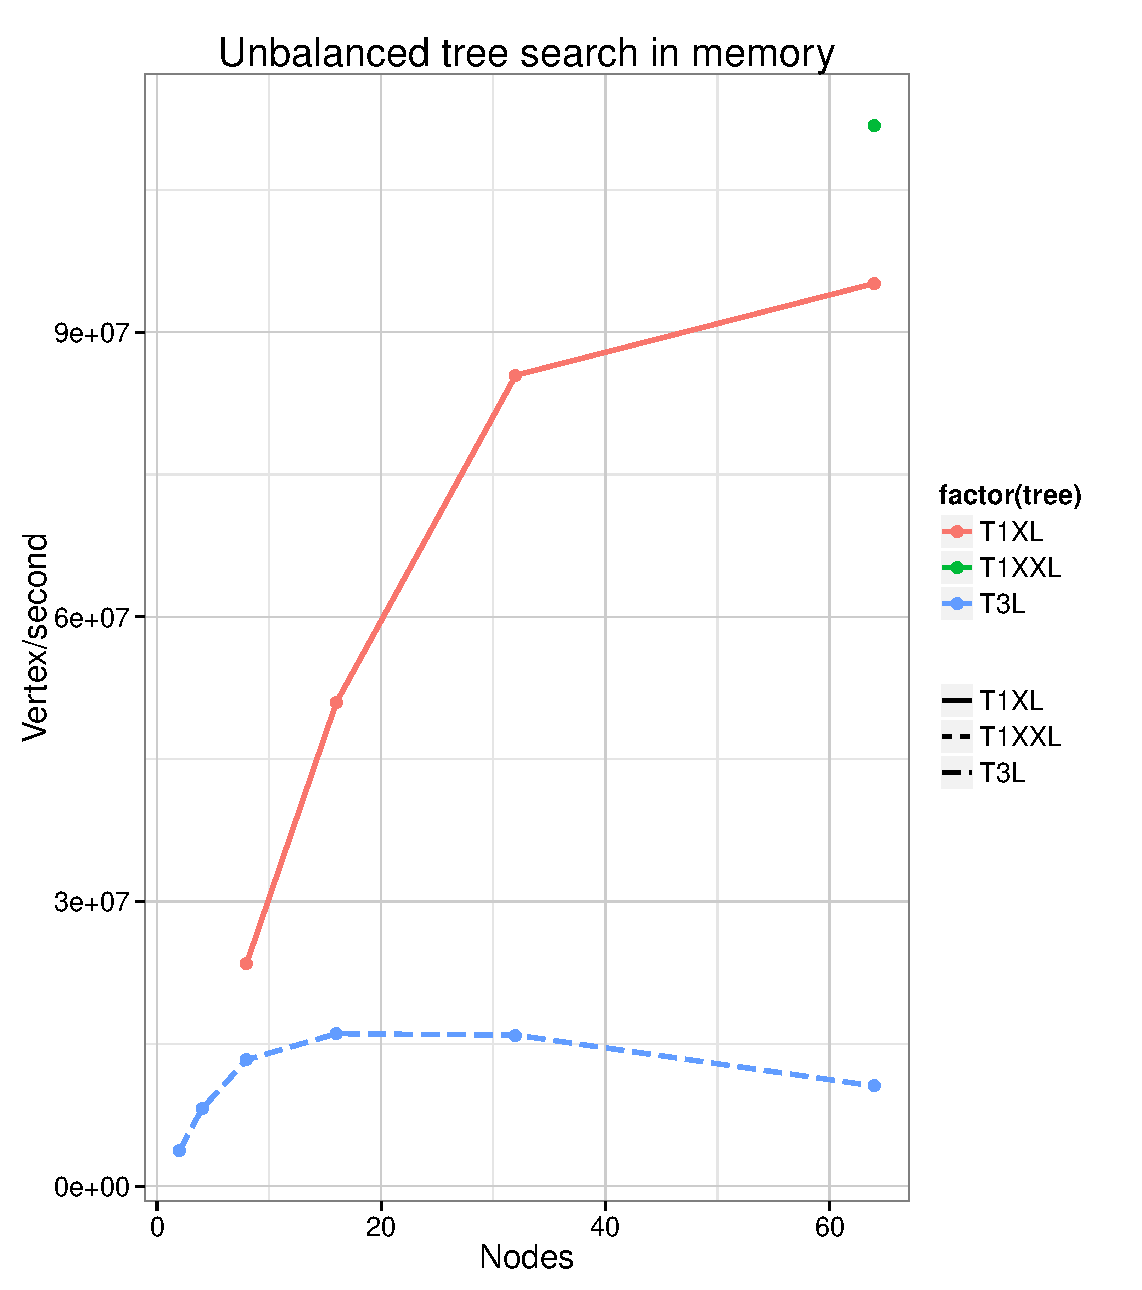
\includegraphics[width=0.5\textwidth]{figs/uts_scale.pdf}
    \end{center}
    \caption{Performance of in-memory unbalanced tree search.}
    \label{fig:uts_compare}
\end{figure}

We ran UTS-mem with a geometric 100M-vertex tree
(T1L). Figure~\ref{fig:uts_compare} shows the performance in terms of
number of vertices visited per second versus number of compute
nodes. \Grappa is 3.2 times faster than the XMT at 16 nodes.  As we will show later, the performance advantage \Grappa has over XMT increases as more nodes are added.  The main reason \Grappa performs better is the software-based delegate synchronization obviates the need for the retry-based synchronization that XMT uses.

\subsubsection{Breadth First Search}\TODO{rewrite with new results}
\begin{figure}[tH]
\begin{center}
  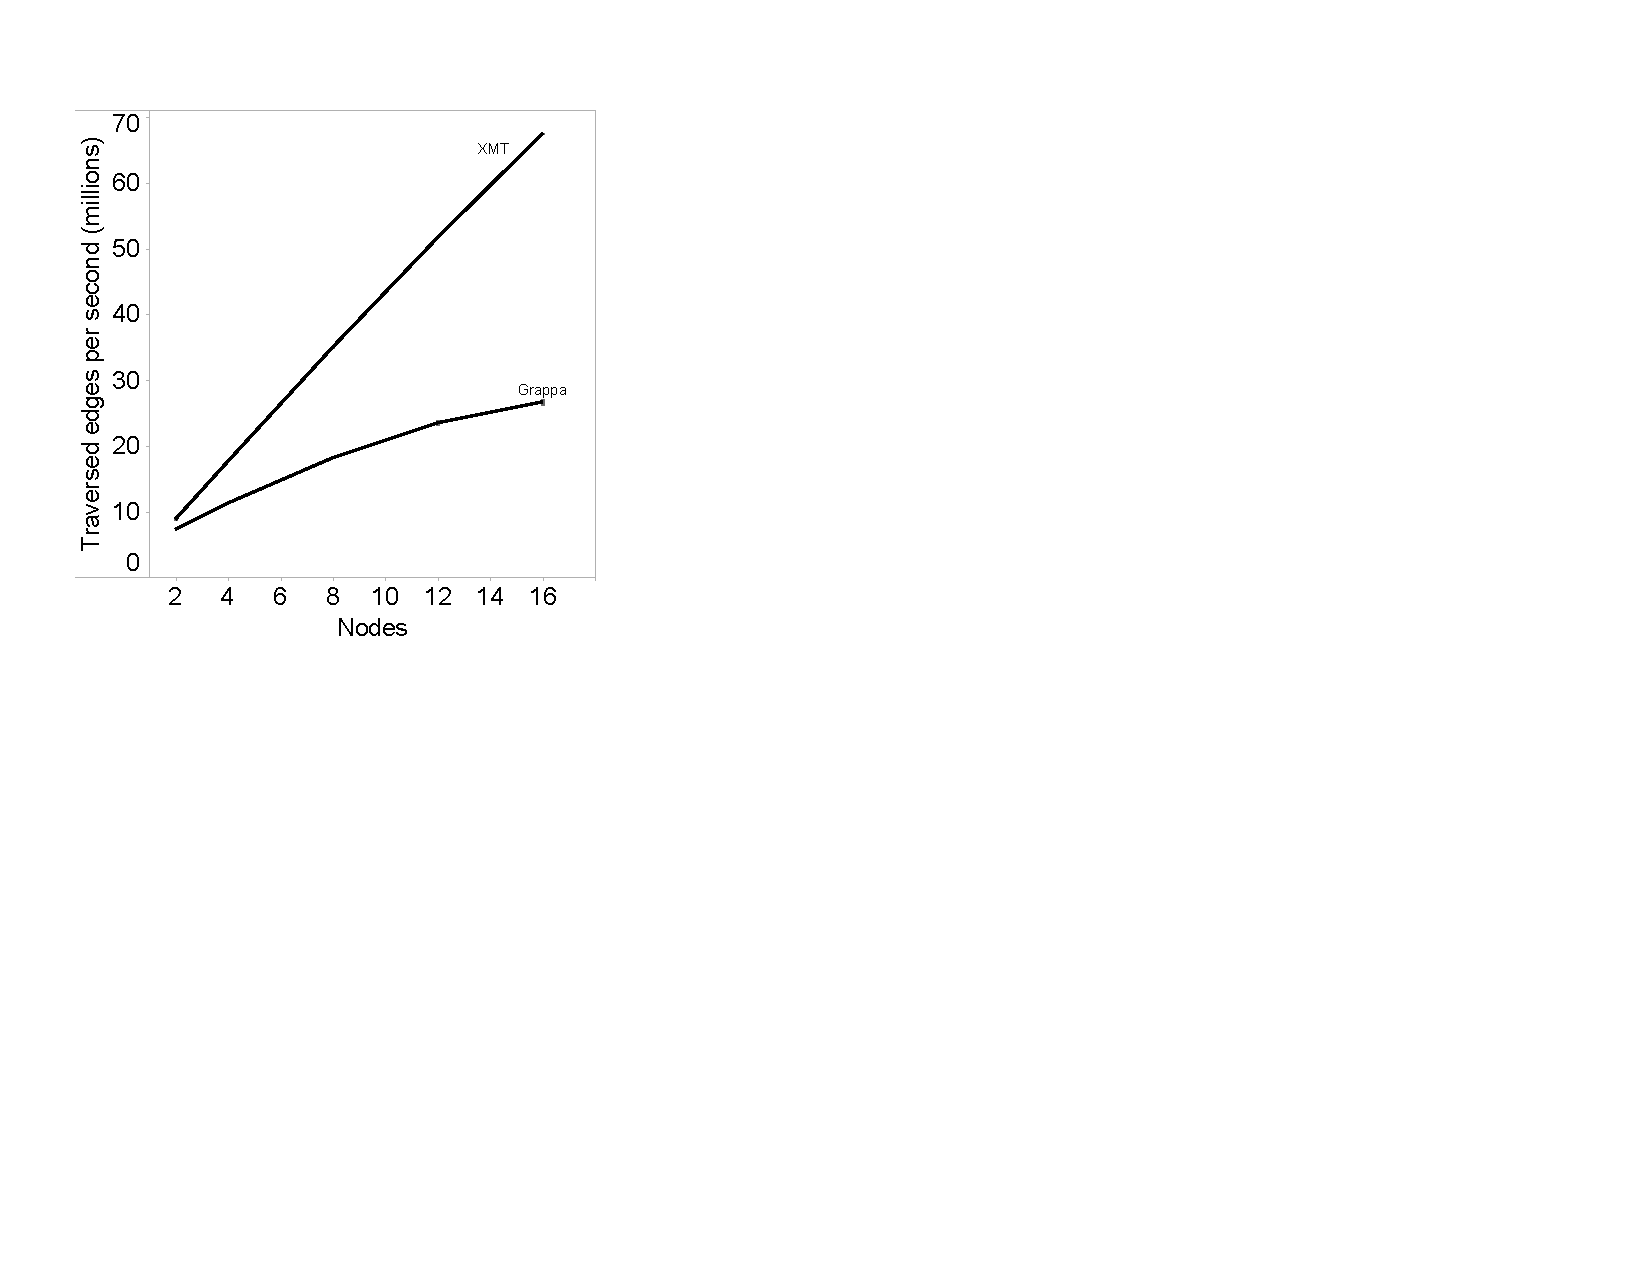
\includegraphics[width=0.95\columnwidth]{figs/bfs_performance}
\begin{minipage}{0.95\columnwidth}
  \caption{\label{fig:bfs-performance} BFS performance}
\end{minipage}
\vspace{-3ex}
\end{center}
\end{figure}

We ran BFS on a synthetic Kronecker graph with $2^{25}$ vertices and
$2^{29}$ edges (25 GB of data). Figure~\ref{fig:bfs-performance} shows
our performance in terms of graph edges traversed per second. The XMT
is 2.5 times faster than \Grappa at 16 nodes.  Performance does scale at a constant rate for \Grappa, suggesting that adding more nodes will increase performance.

\subsubsection{Approximate Betweenness Centrality}\TODO{rewrite with new results}
\begin{figure}[tH]
\begin{center}
  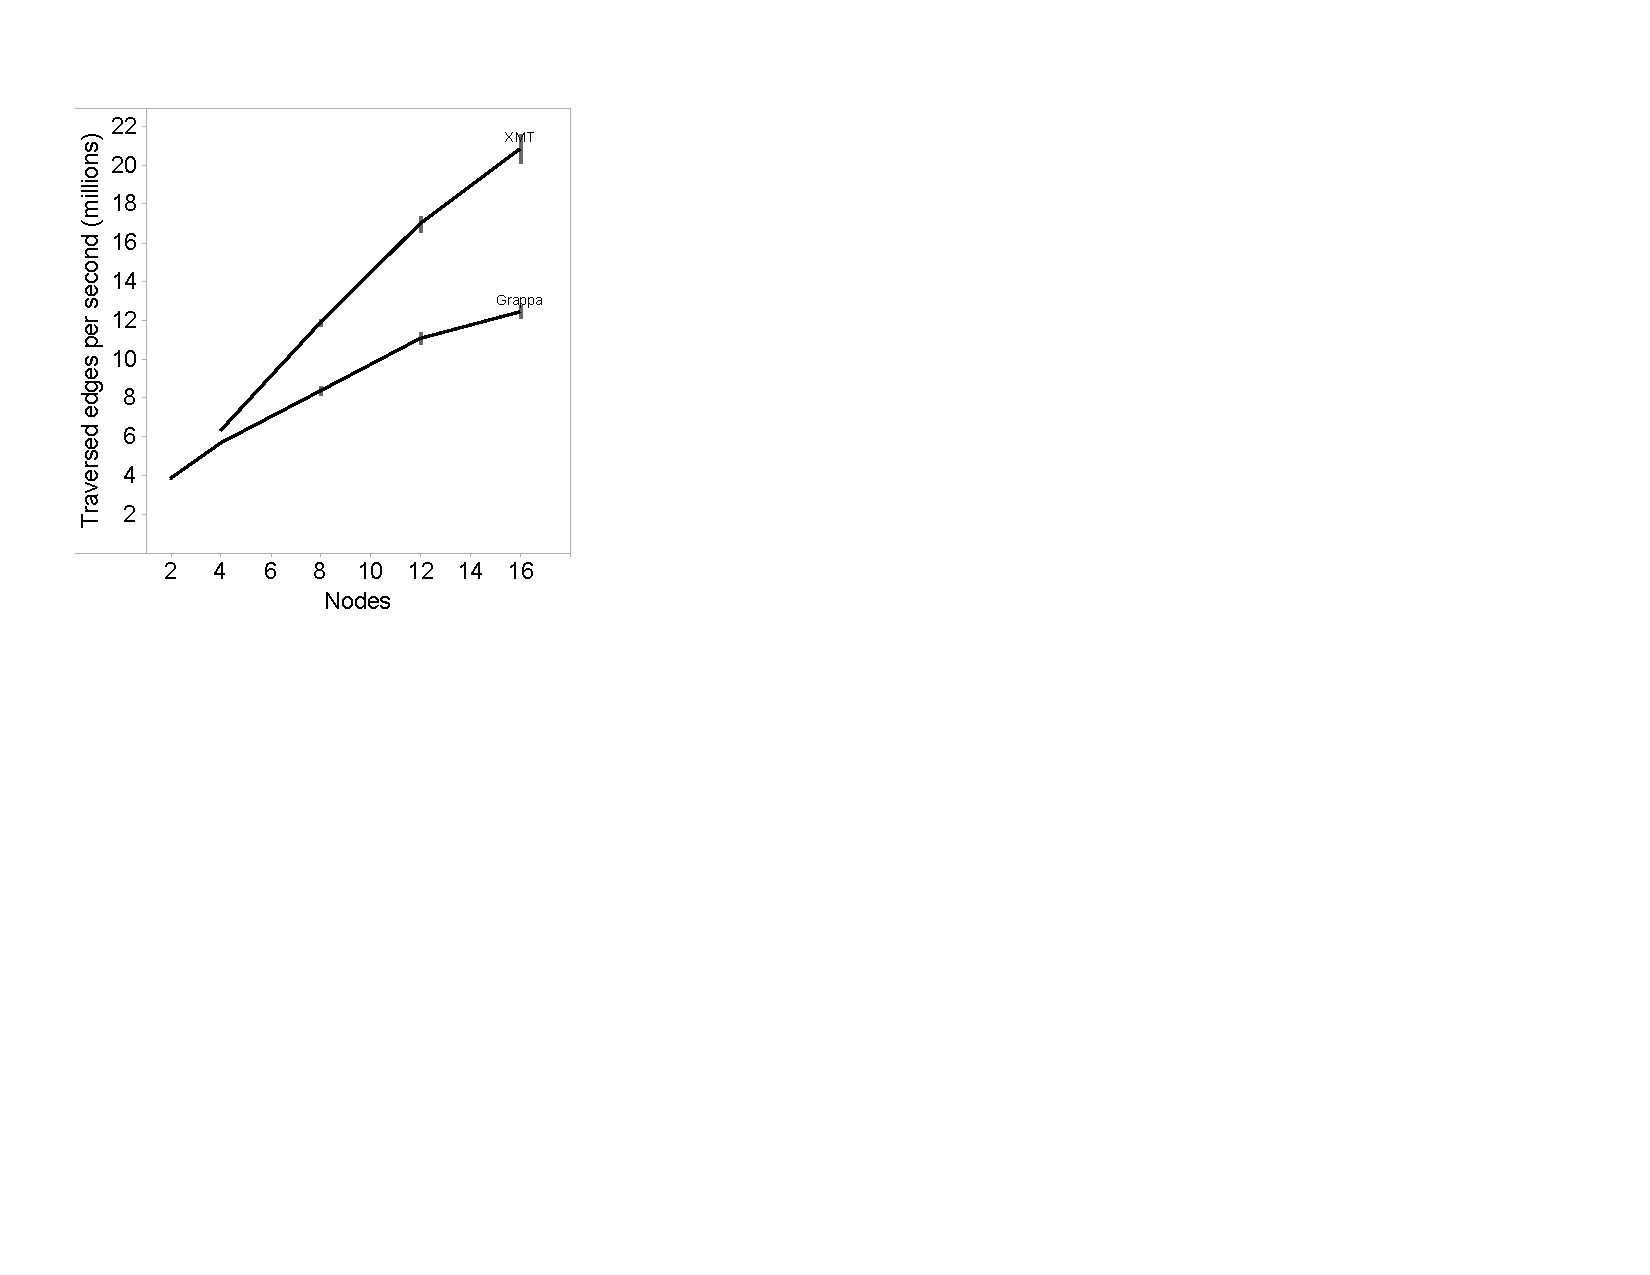
\includegraphics[width=0.95\columnwidth]{figs/centrality_performance}
\begin{minipage}{0.95\columnwidth}
  \caption{\label{fig:centrality-performance} Centrality performance}
\end{minipage}
\vspace{-3ex}
\end{center}
\end{figure}

We ran Betweenness Centrality on the same scale 25 Kronecker graph as
we did for BFS. Figure~\ref{fig:centrality-performance} shows our
performance in terms of graph edges traversed per second. At 16 XMT
processors/cluster nodes, the XMT is 1.75 times faster than \Grappa.

% Got rid of this discussion of UTS by itself, tried to work the highlights in below
%\paragraph{UTS-Mem}
%We ran UTS-Mem on \Grappa and the XMT with a geometric 1.6B-vertex tree
%(T1XL) and a geometric 4.2B-vertex tree (T1XXL), using up to 128
%nodes---the maximum we had available for each. \Grappa results are for 5 cores per node. \Grappa with 20 machines is faster than the entire XMT of 128 processors.

%\Grappa achieves \checkme{188Mvert/s} with 128 nodes and the XMT
%achieves only 50Mvert/s, plateauing at 60 nodes. Beyond 90 nodes, \Grappa adds 1.4 Mvert/s/node.
%The XMT scales at 850 Kvert/s/node, until it plateaus. \Grappa keeps
%scaling up through 128 nodes, although scaling
%declines because of the unscalability of our aggregation mechanism as
%number of network endpoints increases. 
%
%Despite our efforts to tune the UTS implementation specific to the 
%XMT, performance does not scale well with increasing processor count,
%flattening out around 60 processors.  When we increase the size of
%the tree from 100M to 4.2B, we find that performance does not improve,
%suggesting that performance is not limited by task parallelism.
%Cray's performance tools show an increasing number of memory
%retry operations for failed synchronization operations generated by
%the runtime, which create network contention.
%
To determine how \Grappa's performance scales compared to the performance of the entire XMT, we ran a set of experiments up to all 128 XMT processors and 128 cluster nodes. For the XMT, the number of allowed processors was varied up to the entire machine, with some minor tuning of stream parameters needed to get optimal performance. For \Grappa, parameters such as cores per node, aggregator timeouts, and parallel threshold were tuned to get the best performance for each node count. All of the benchmarks continue to improve out to 128 nodes for \Grappa. UTS continues to fare better than the XMT with large node counts, with the XMT appearing to plateau at 60 processors due to contention from synchronization retries, while \Grappa handles this by suspending tasks until messages return. For BFS and Centrality, the XMT scales approximately a constant factor better than \Grappa. We attribute this to a limitation in the current aggregator design and network stack that \Grappa uses.  This limits the practical number of cores we can use to 6 per node (adding more cores per node \emph{decreases} performance).  Ironically, this limitation makes \Grappa applications compute-bound instead of network-bound.  Work is ongoing to rework the Infiniband driver stack and aggregation interface to remove this limitation and improve aggregation addressing using local routing.

\begin{figure}[ht]
    \begin{center}
      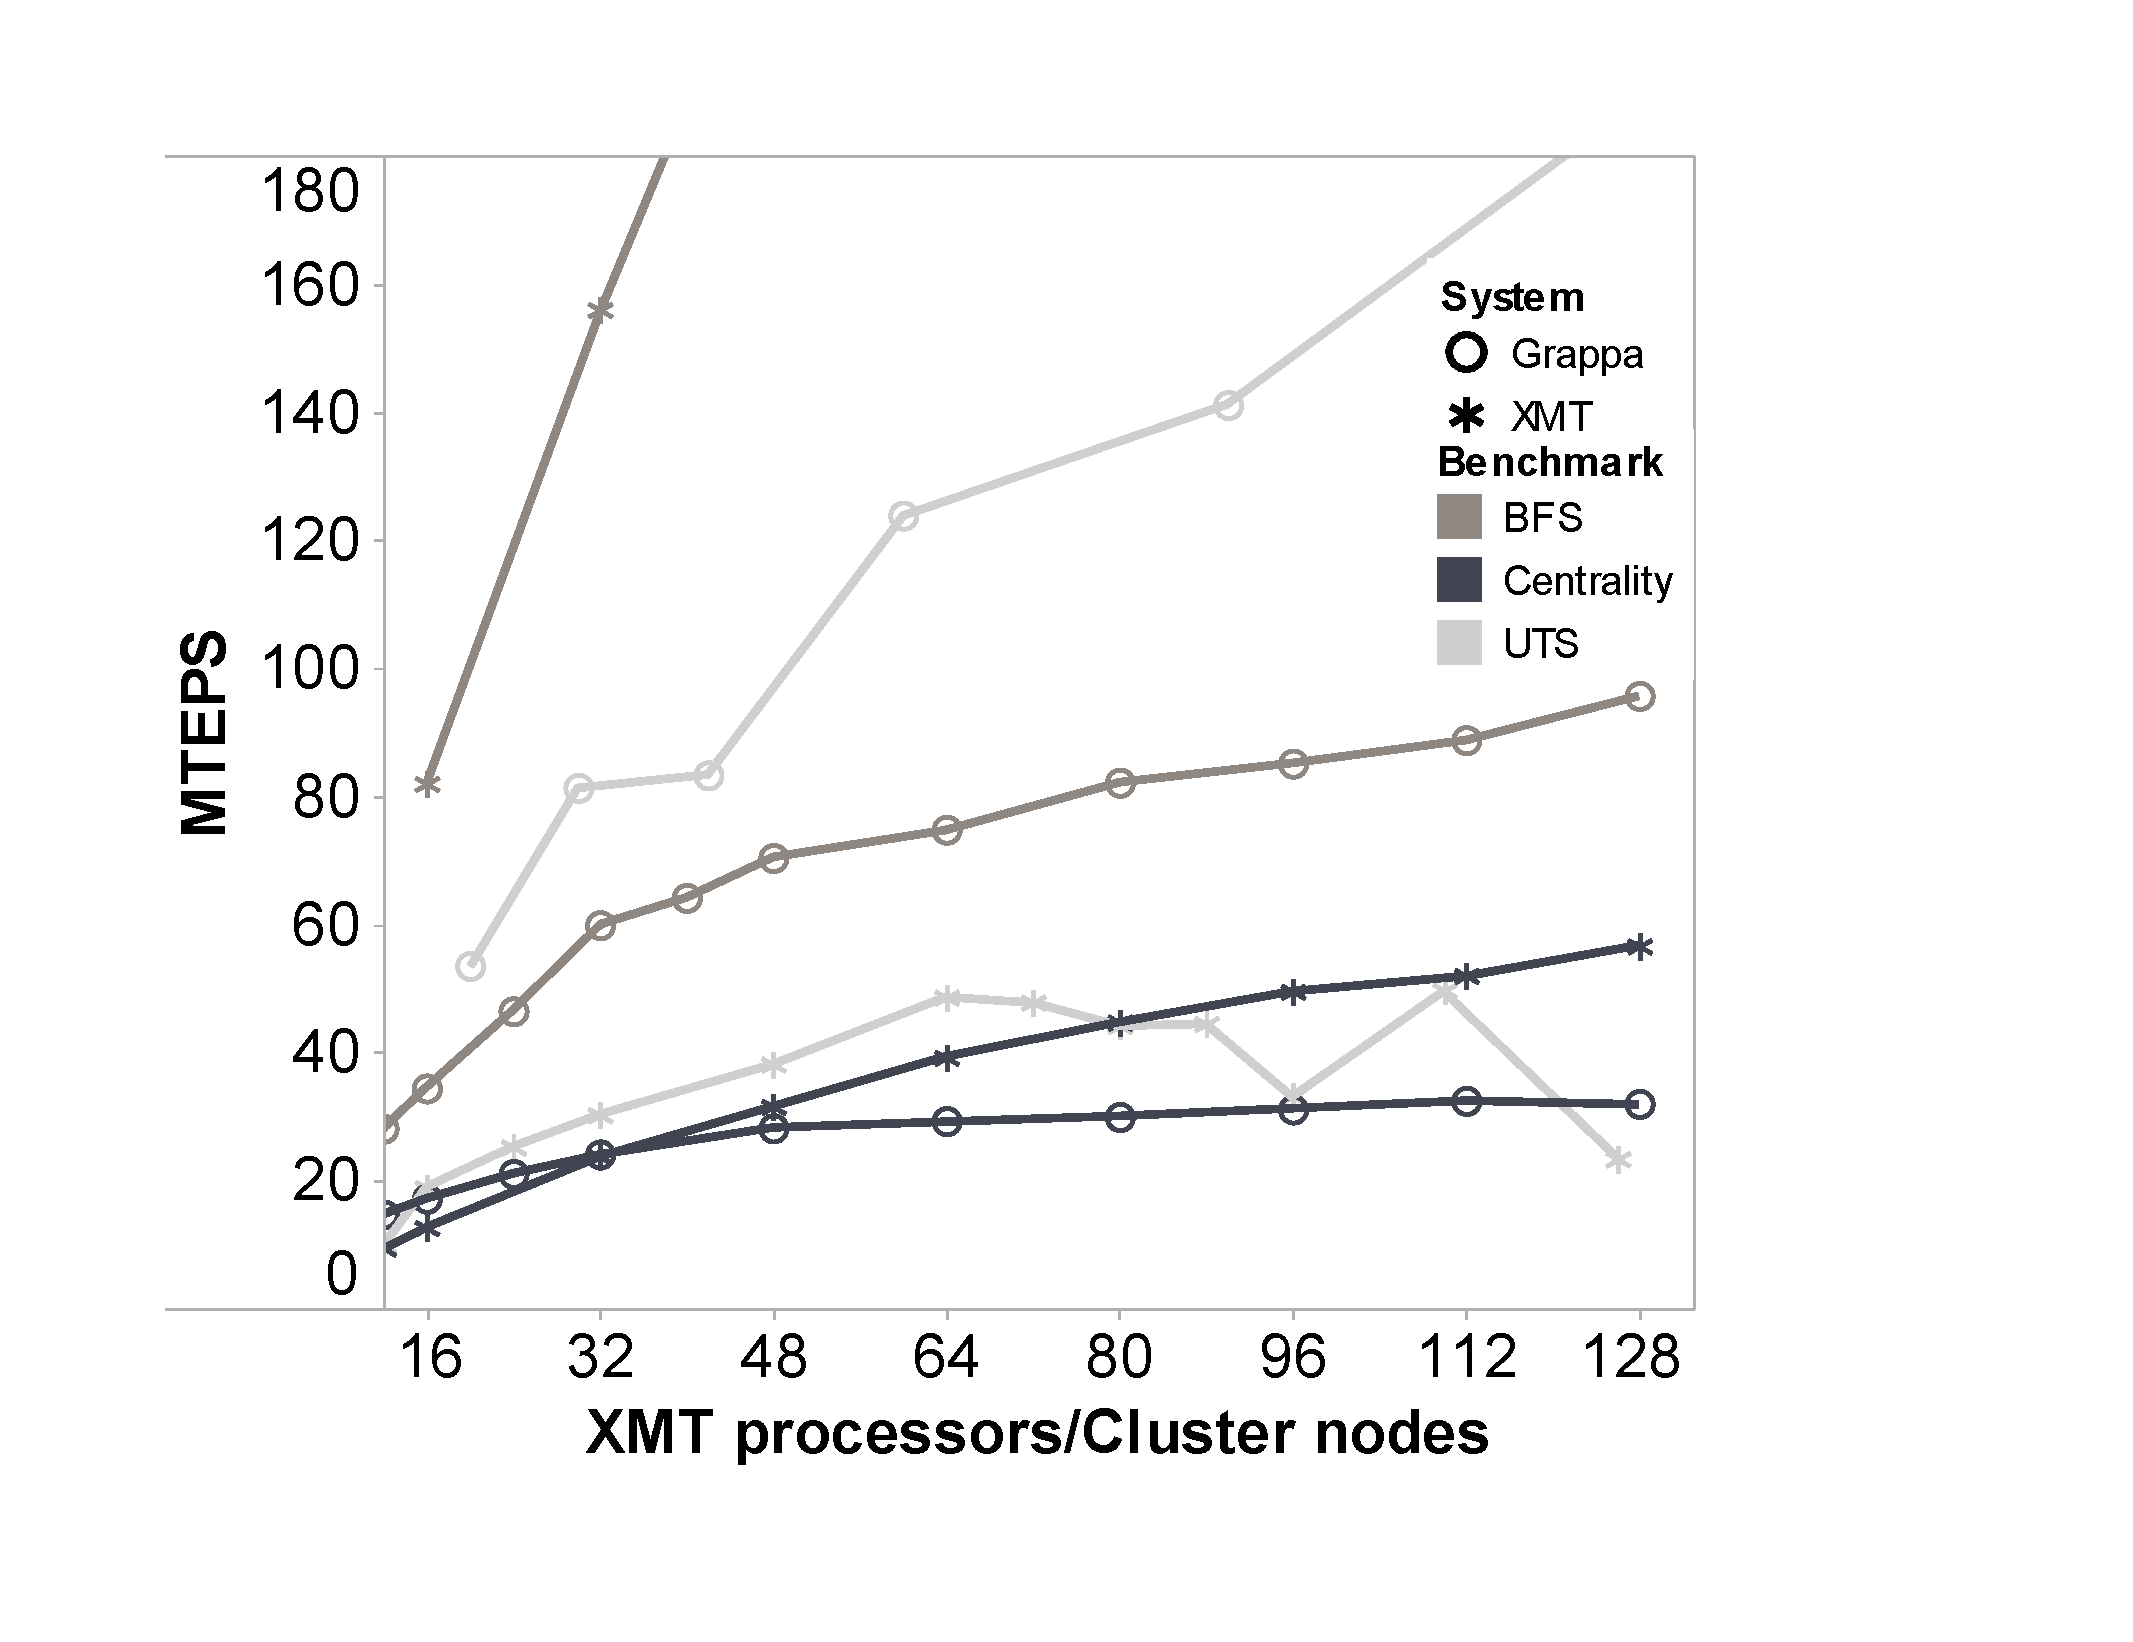
\includegraphics[width=0.5\textwidth]{figs/scaling_cropped.pdf}
    \end{center}
    \caption{Scaling number of nodes: \Grappa continues to perform significantly better than XMT for UTS but scales a constant factor slower than XMT for BFS (4x slower) and Centrality (2x slower). }
    \label{fig:uts_threshold}
\end{figure}

\subsection{Scaling}\label{sec:scaling} \TODO{rewrite with new results}

\subsubsection{Network Aggregation Performance and Robustness}

\begin{figure}[htb]
\begin{center}
  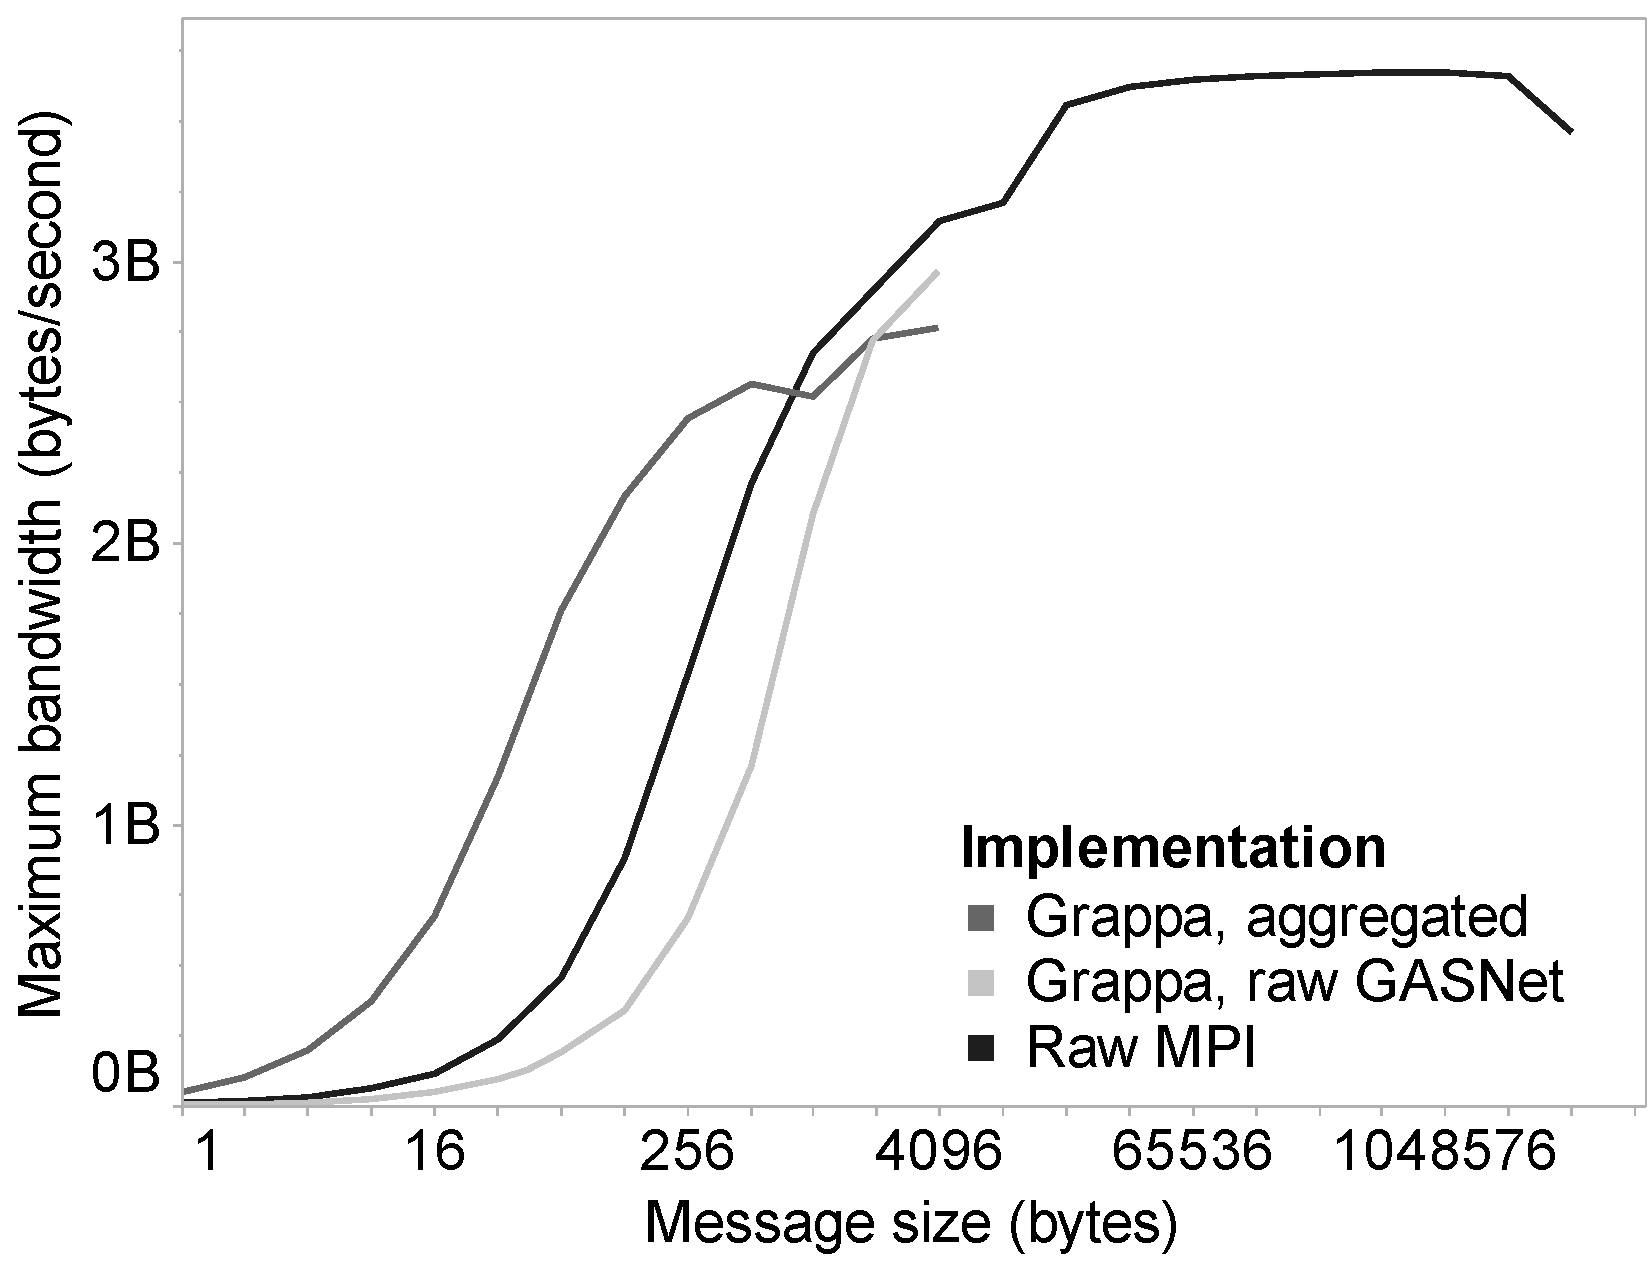
\includegraphics[width=0.95\columnwidth]{figs/aggregator_ping}
\begin{minipage}{0.95\columnwidth}
  \caption{\label{fig:aggregator-ping} Bandwidth versus message size
    unidirectional ping test for \Grappa with aggregation, \Grappa with
    raw GASNet messages, and MPI. Aggregation provides an 11x
    bandwidth benefit at our common operating point.}
\end{minipage}
\vspace{-3ex}
\end{center}
\end{figure}

To evaluate the benefits of network aggregation, we ran two experiments.
First, we ran a simple unidirectional ping test to see the maximum
benefit the aggregator can provide in terms of improved network
efficiency. Second, we ran BFS with the aggregator disabled in order to
measure its benefit on an application.

To implement the ping test, we wrote a simple \Grappa application where
the cores of one node send messages as fast as possible to the cores
of another node. We vary the size of the payload up the maximum
payload size supported by the aggregator (nearly 4KB). Each core has a
single task sending to a single destination, so this is a best case
scenario for the aggregator. To see the benefit of the aggregator, we
added a bypass that lets us send messages directly through GASNet. We
also compare against the OSU \texttt{osu\_mbw\_mr} benchmark
\cite{osu:mpi}  compiled against OpenMPI 1.5.3; this
benchmark has the same pattern of communication but doesn't have the
overhead of \Grappa's context switching.

The results are shown in Figure~\ref{fig:aggregator-ping}. There are
two key observations.

First, small message performance against the existing libraries is, as expected, poor. The MPI application test shows us that peak per node
bandwidth supported by our infiniband card is 3.4GB/s. This is
achievable only with large messages; we must send 16KB packets to get
within 5 percent of peak bandwidth. But in our benchmarks, we saw
average message between 32 and 64 bytes. At 32 bytes, the MPI test is
using less than 7 percent of its peak bandwidth. \Grappa sending
messages directly through GASNet uses less than 3 percent of the peak
bandwidth.

Second, aggregation has the potential to improve this situation by an
order of magnitude. With aggregation, \Grappa is able to send 32-byte
messages over 12 times faster than using GASNet directly. This is a
more respectable 32 percent of peak bandwidth. Due to expedient design
decisions, \Grappa's aggregator limits its aggregation to 4KB; this
limits its peak achievable bandwidth to 75 percent of the actual
peak.

This comparison is the best possible case for the aggregator. In
order to verify that the aggregator still has value on actual
applications at scale, we ran a small (100M node tree) UTS-Mem
with the aggregator disabled, on 16 nodes.
Figure~\ref{fig:no-aggregation-uts}. At this configuration, the aggregator
improves our application performance by 10x. 

\begin{figure}[htb]
\begin{center}
  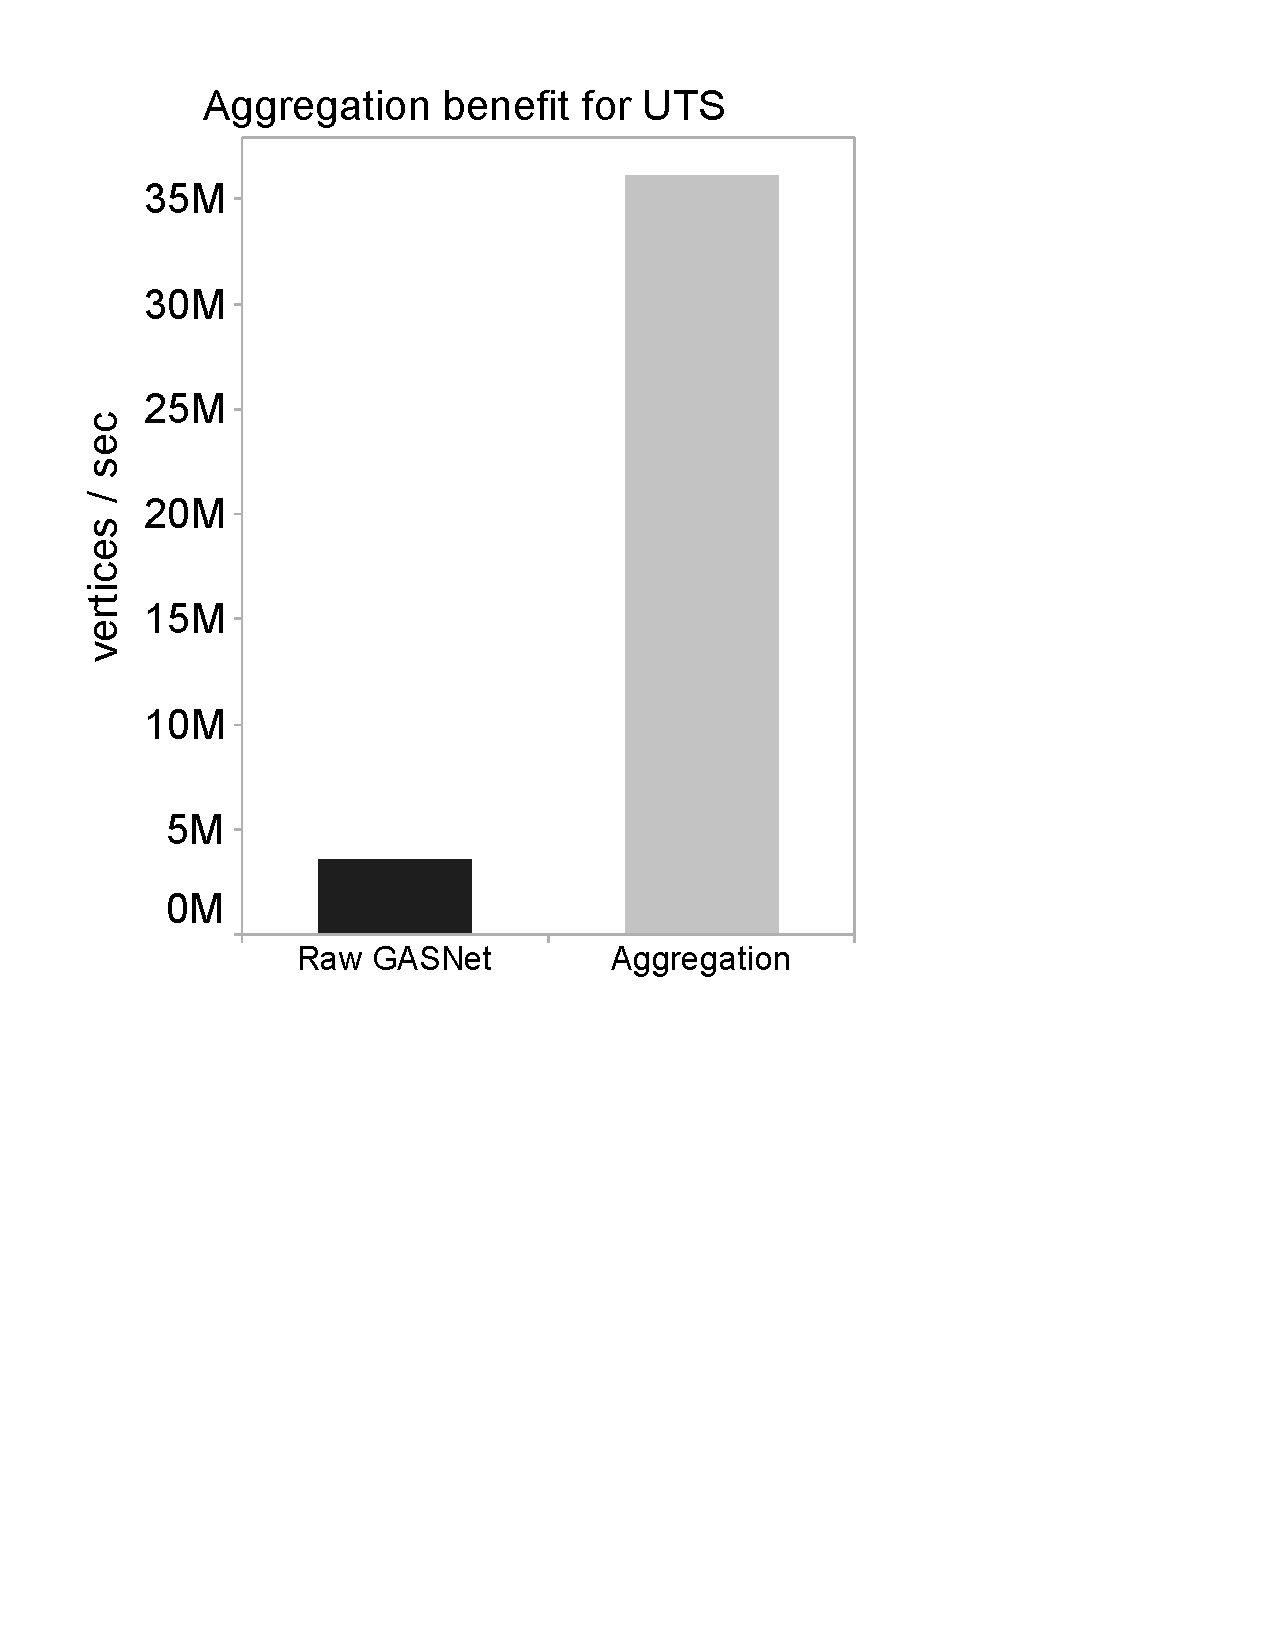
\includegraphics[width=0.95\columnwidth]{figs/no_aggregation_uts.pdf}
\begin{minipage}{0.95\columnwidth}
  \caption{\label{fig:no-aggregation-uts} Performance of UTS on 16
      nodes with and without \Grappa's aggregation.}
\end{minipage}
\vspace{-3ex}
\end{center}
\end{figure}

\subsection{Scaling}
% Got rid of this discussion of UTS by itself, tried to work the highlights in below
%\paragraph{UTS-Mem}
%We ran UTS-Mem on \Grappa and the XMT with a geometric 1.6B-vertex tree
%(T1XL) and a geometric 4.2B-vertex tree (T1XXL), using up to 128
%nodes---the maximum we had available for each. \Grappa results are for 5 cores per node. \Grappa with 20 machines is faster than the entire XMT of 128 processors.
%\Grappa achieves \checkme{188Mvert/s} with 128 nodes and the XMT
%achieves only 50Mvert/s, plateauing at 60 nodes. Beyond 90 nodes, \Grappa adds 1.4 Mvert/s/node.
%The XMT scales at 850 Kvert/s/node, until it plateaus. \Grappa keeps
%scaling up through 128 nodes, although scaling
%declines because of the unscalability of our aggregation mechanism as
%number of network endpoints increases. 
%
%Despite our efforts to tune the UTS implementation specific to the 
%XMT, performance does not scale well with increasing processor count,
%flattening out around 60 processors.  When we increase the size of
%the tree from 100M to 4.2B, we find that performance does not improve,
%suggesting that performance is not limited by task parallelism.
%Cray's performance tools show an increasing number of memory
%retry operations for failed synchronization operations generated by
%the runtime, which create network contention.
%
To determine how \Grappa's performance scales compared to the performance of the entire XMT, we ran a set of experiments up to all 128 XMT processors and 128 cluster nodes. For the XMT, the number of allowed processors was varied up to the entire machine, with some minor tuning of stream parameters needed to get optimal performance. For \Grappa, parameters such as cores per node, aggregator timeouts, and parallel threshold were tuned to get the best performance for each node count. All of the benchmarks continue to improve out to 128 nodes for \Grappa. UTS continues to fare better than the XMT with large node counts, with the XMT appearing to plateau at 60 processors due to contention from synchronization retries, while \Grappa handles this by suspending tasks until messages return. For BFS and Centrality, the XMT scales approximately a constant factor better than \Grappa. We attribute this to a limitation in the current aggregator design and network stack that \Grappa uses.  This limits the practical number of cores we can use to 6 per node (adding more cores per node \emph{decreases\/} performance).  Ironically, this limitation makes \Grappa applications compute-bound instead of network-bound.  Work is ongoing to rework the Infiniband driver stack and aggregation interface to remove this limitation and improve aggregation addressing using local routing.

\begin{figure}[ht]
    \begin{center}
      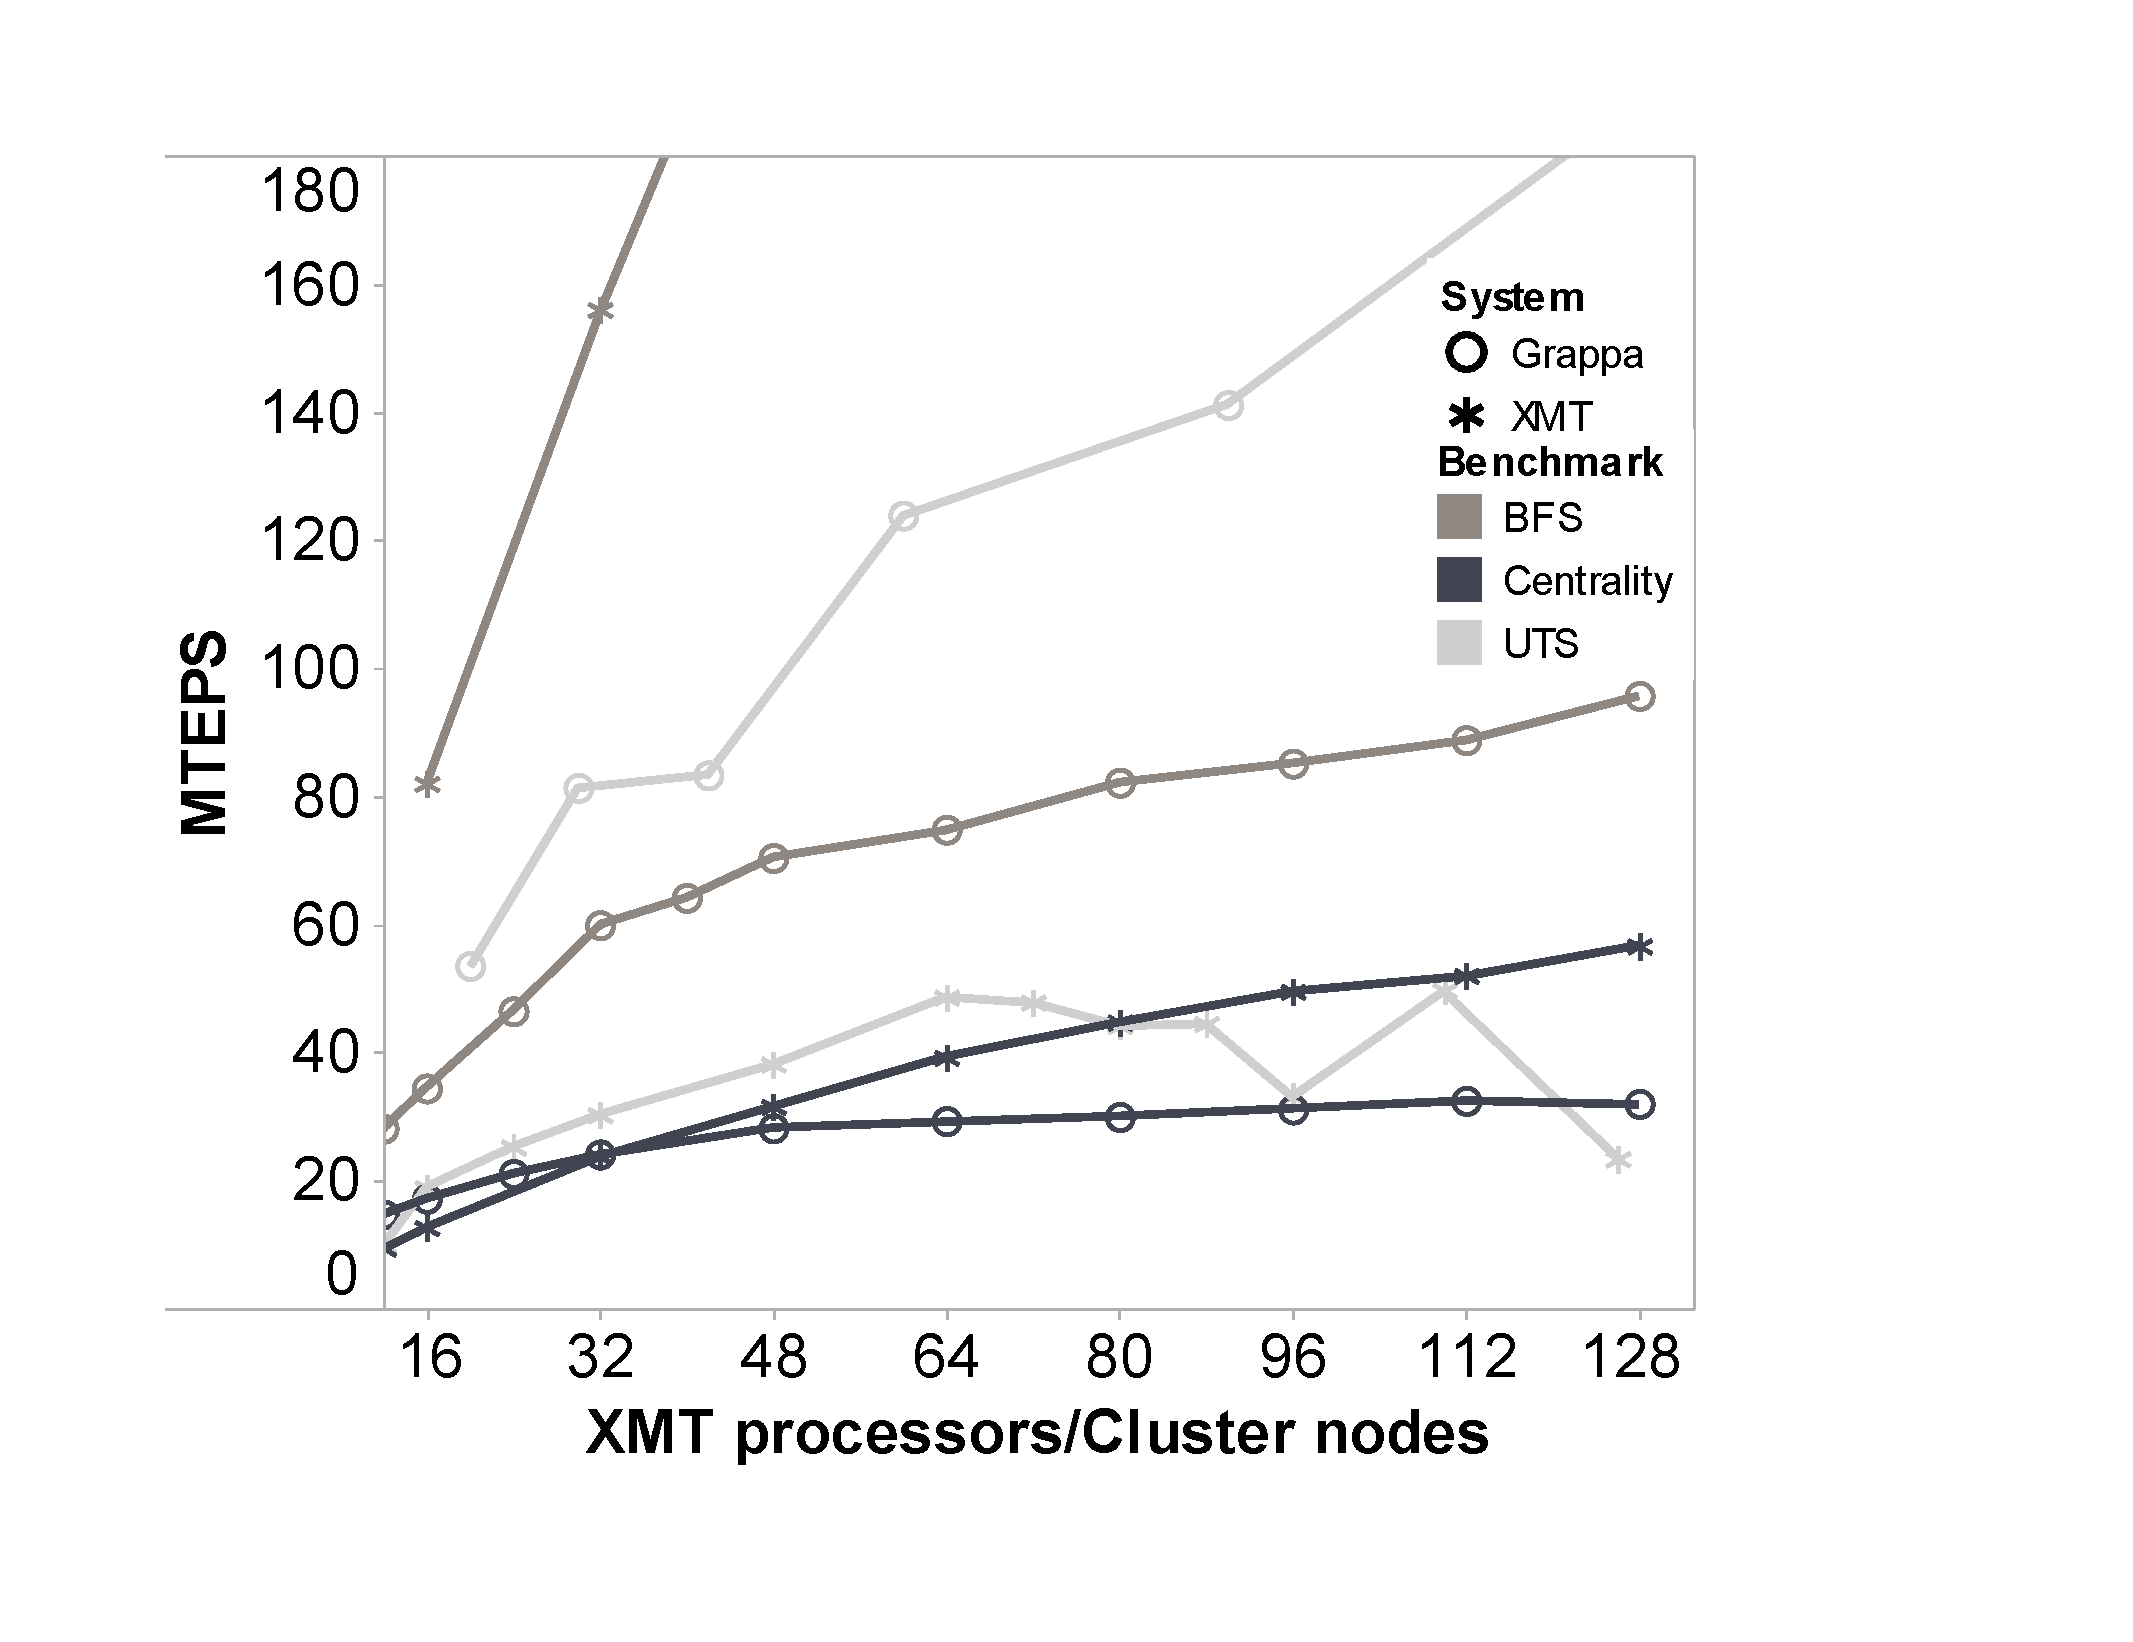
\includegraphics[width=0.5\textwidth]{figs/scaling_cropped.pdf}
    \end{center}
    \caption{Scaling number of nodes: \Grappa continues to perform significantly better than XMT for UTS but scales a constant factor slower than XMT for BFS (4x slower) and Centrality (2x slower). }
    \label{fig:uts_threshold}
\end{figure}


\subsection{Sensitivity}

\paragraph{Aggregator timeout}

\begin{figure}[htb]
\begin{center}
  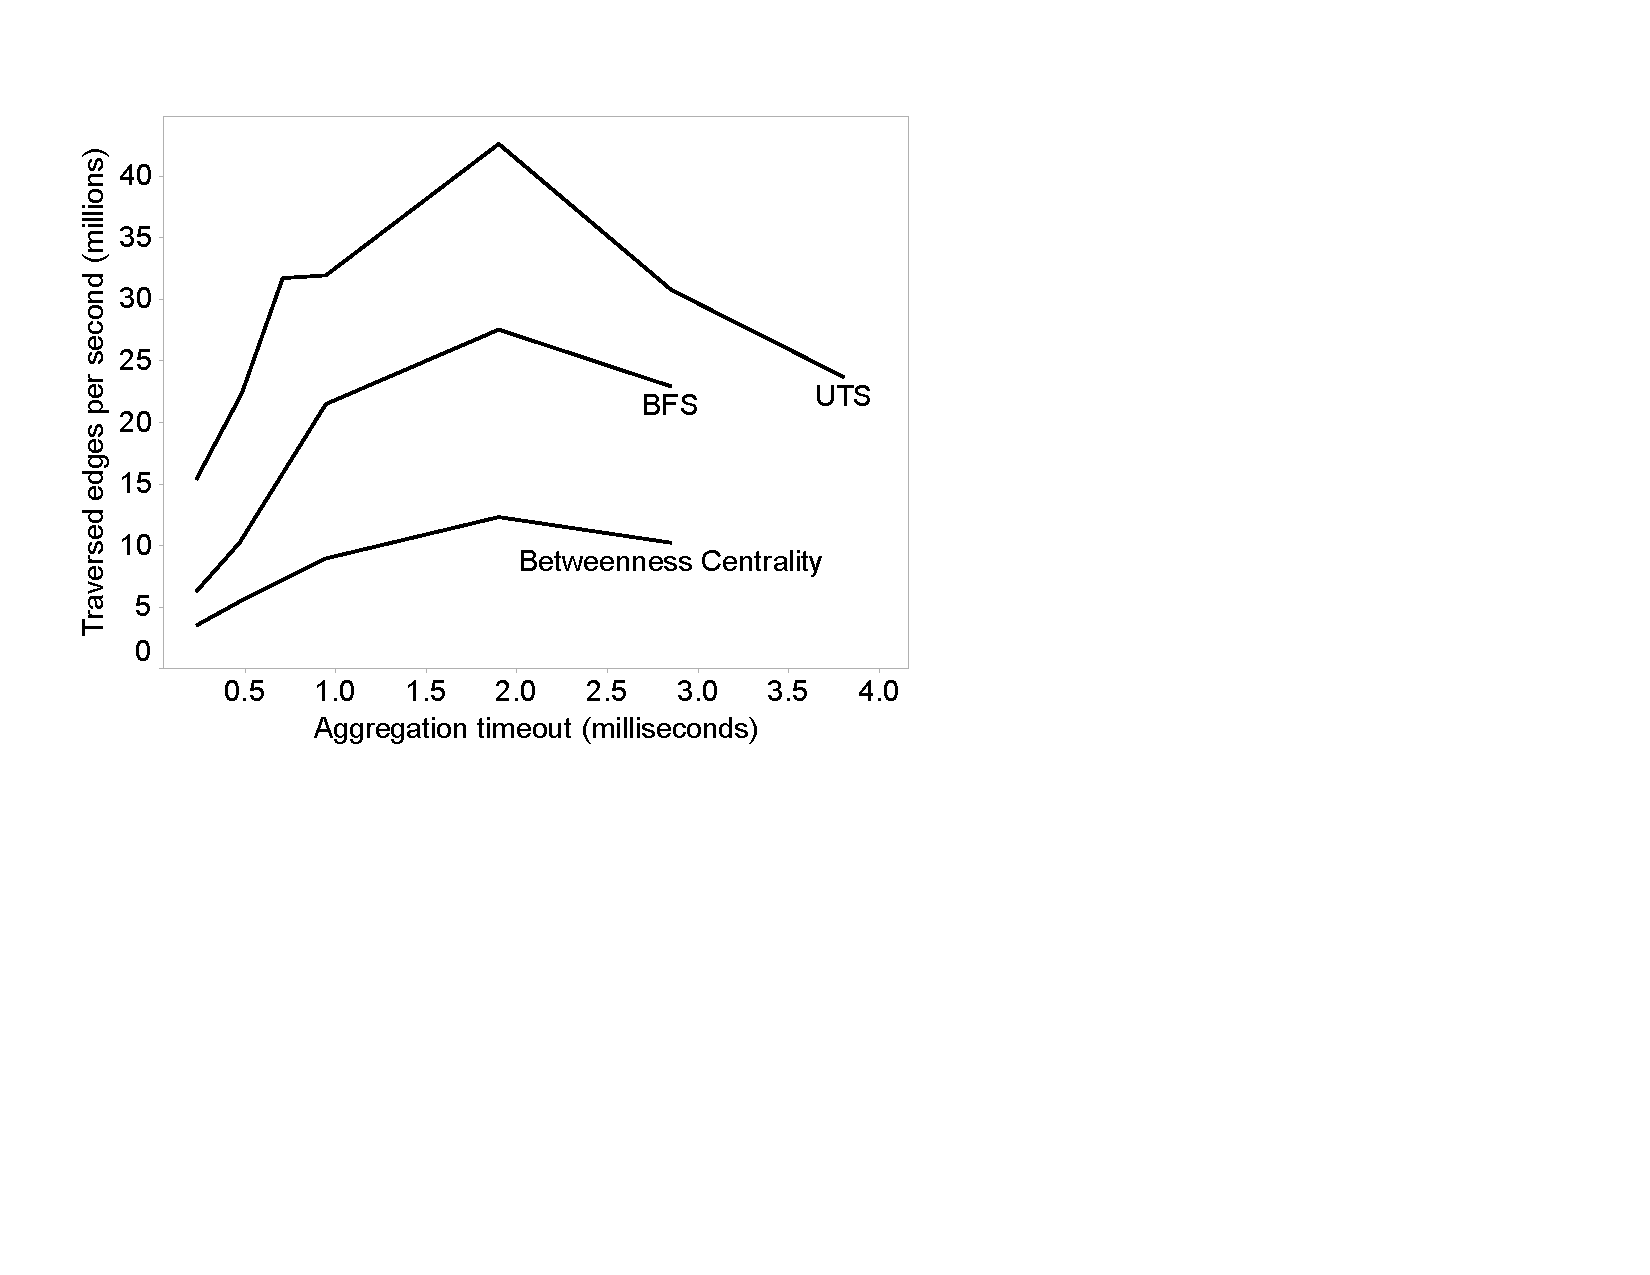
\includegraphics[width=0.95\columnwidth]{figs/flushticks_sweep}
\begin{minipage}{0.95\columnwidth}
  \caption{\label{fig:bfs-sweep-flushticks} Sensitivity to aggregation delay}
\end{minipage}
\vspace{-3ex}
\end{center}
\end{figure}


One of the key parameters of the aggregator is the message
timeout. All messages that are queued must eventually be sent in order
to ensure progress. In the best case, we are able to aggregate enough
messages to fill an aggregation buffer and cause it to be sent, but as
we scale up, the average rate of messages heading to a common
destination decreases, and this gets harder. To bound the problem, the
aggregator includes a timeout. Any packet waiting this long is sent
the next time the communications layer is serviced.

Figure~\ref{fig:bfs-sweep-flushticks} shows a sweep of this parameter
for UTS, BFS, and Betweenness Centrality on 16 nodes, using the
datasets described previously. The maximum number of workers is fixed
at 2048. All the benchmarks show a performance peak with a 2
millisecond timeout; at this point we are delaying long enough to
aggregate the largest packets we can; setting the parameter higher
causes tasks to wait longer for responses, but few new requests are
being generated.


\begin{figure}[htb]
\begin{center}
  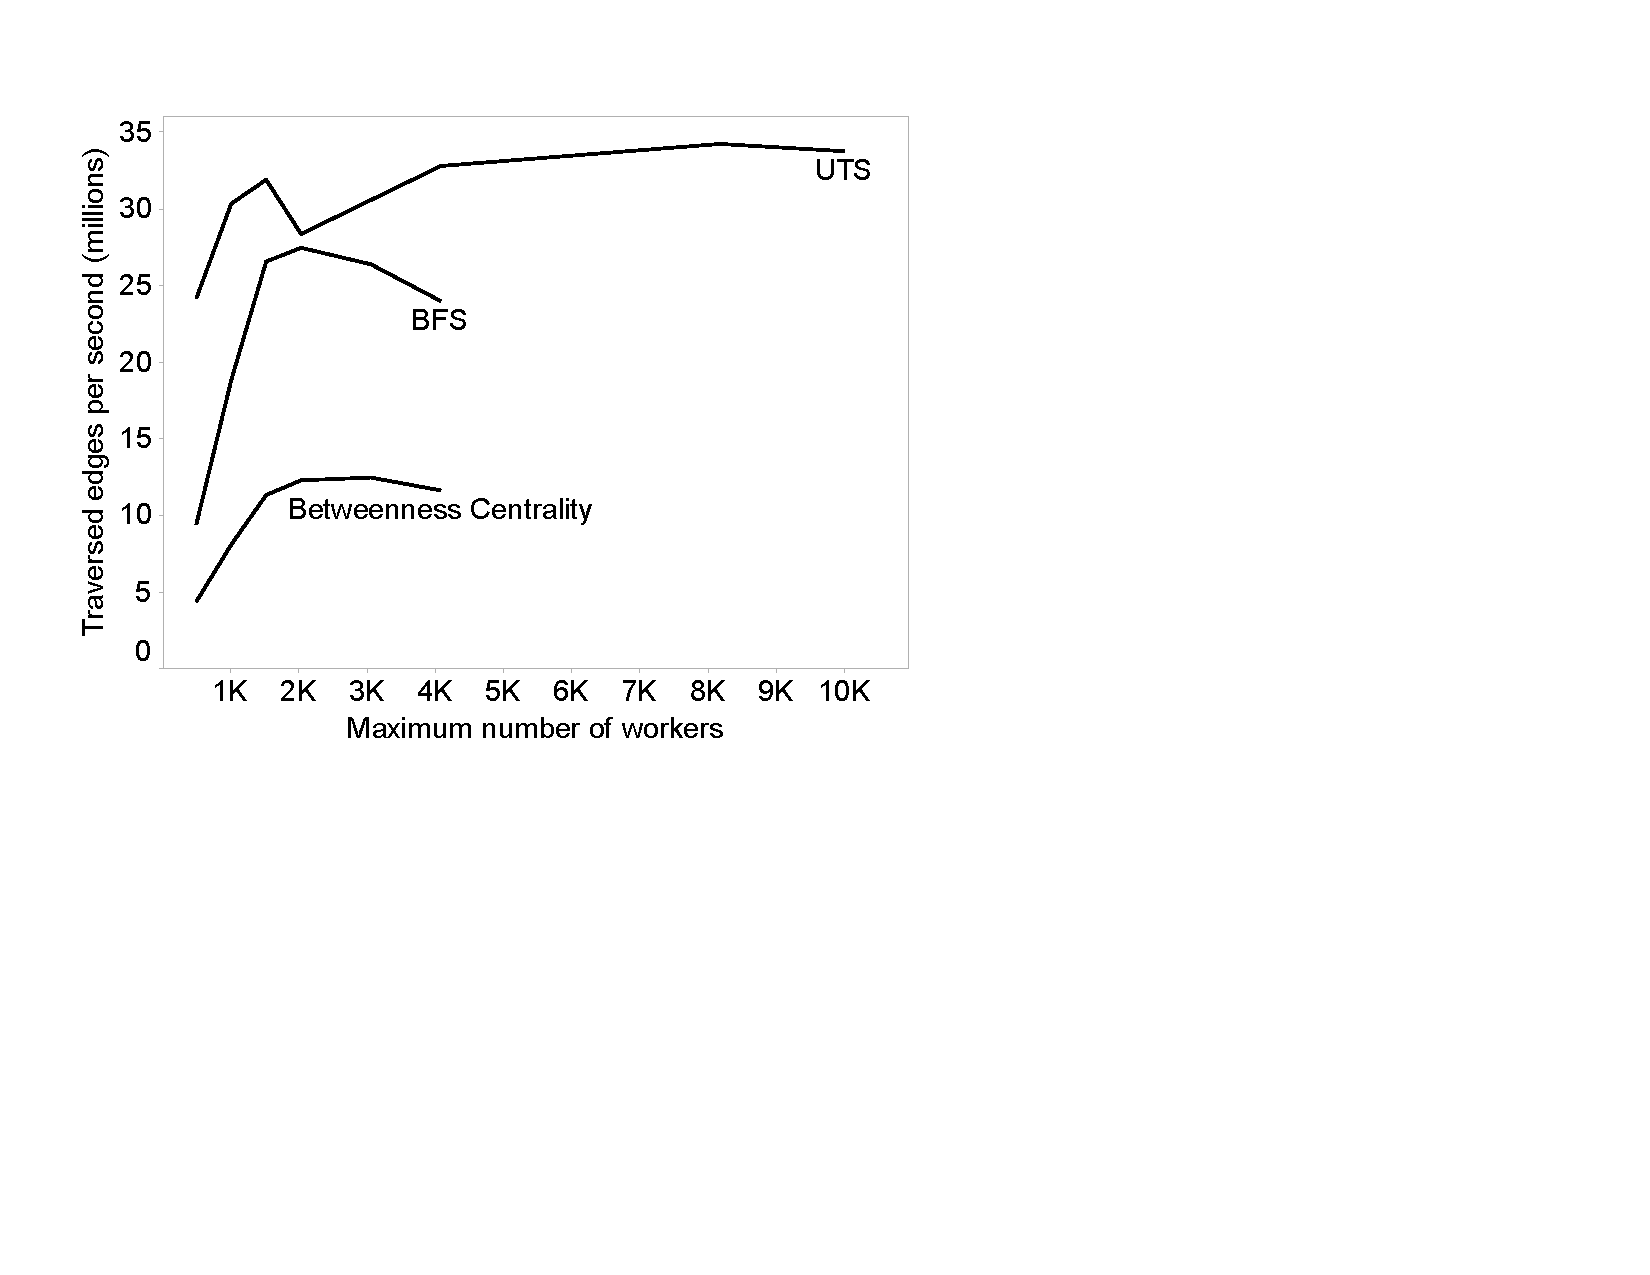
\includegraphics[width=0.95\columnwidth]{figs/worker_sweep}
\begin{minipage}{0.95\columnwidth} 
  \caption{\label{fig:bfs-sweep-workers} Sensitivity to maximum active tasks}
\end{minipage}
\vspace{-3ex}
\end{center}
\end{figure}

\subsubsection{Number of active tasks} \TODO{possibly eliminate}

When a task issues a request that requires a response, it blocks to
allow other tasks to utilize its core. These tasks may also block. To
support the many milliseconds of latency aggregation adds, we need to
support many thousands of blocked tasks. One of the key parameters of
the runtime is the number of blocked tasks allowed; we need enough to
cover the network and aggregation latency, but too many running tasks
can add extra latency as they all must be multiplexed onto the same core.

Figure~\ref{fig:bfs-sweep-workers} shows a sweep of the maximum number
of active tasks (workers) per core for each of our three benchmarks on
16 nodes. The aggregator timeout is set at 1 ms for UTS and 2 ms for
BFS and Betweenness Centrality. The performance peak shifts in this
case, with UTS peaking at 1536 workers, BFS peaking at 2048 workers,
and Betweenness Centrality peaking at 3072 workers. This is the point
where we have enough workers to cover the latency of aggreation. The
different values reflect the different amounts of work done by a task
in each benchmark; UTS does the least, while Betweenness Centrality does the most.

%\subsubsection{Work stealing parameters}
%
%\paragraph{Chunk size}
%
%It is important to steal multiple tasks at a time to both amortize the
%cost of stealing over the network and to spread out work quickly in a
%large system. Figure~\ref{fig:ut_chunksize} shows performance and
%stealing statistics for UTS on \checkme{30} nodes as we increase the stealing chunk size. Recall
%that a thief will take a number of tasks equal to the minimum of half
%the available work or the chunk size; steals fail only when the victim
%has fewer than 2 available tasks. As the scheduler is allowed to
%steal more work beyond 1 task, we see that performance increases up to 6x. This
%shows that the heuristic of stealing the oldest task from victims is
%insufficient alone when a tree-structured computation is imbalanced,
%as observed in \cite{UTS}. By observing sampled state in the execution
%trace, we find that a chunk size as low as 1 allows stealing to
%spread the load evenly across the cluster but cores spend much time
%underutilized as multiple workers wait for steal replies that
%utlimately return little new work.
%
%Performance plateaus before maximum steal amount is limited by the
%size of the victim's task queue. This indicates that artificially limiting steals
%to \checkme{128} tasks does not limit performance. Although a lower
%chunk size limits how quickly work spreads, for sufficient chunk size,
%the heuristic of stealing the oldest tasks from victims in tree-based computations allows for
%stolen work to expand quickly.


%% UTS: chunk size
%\begin{figure}[ht]
%    \begin{center}
%      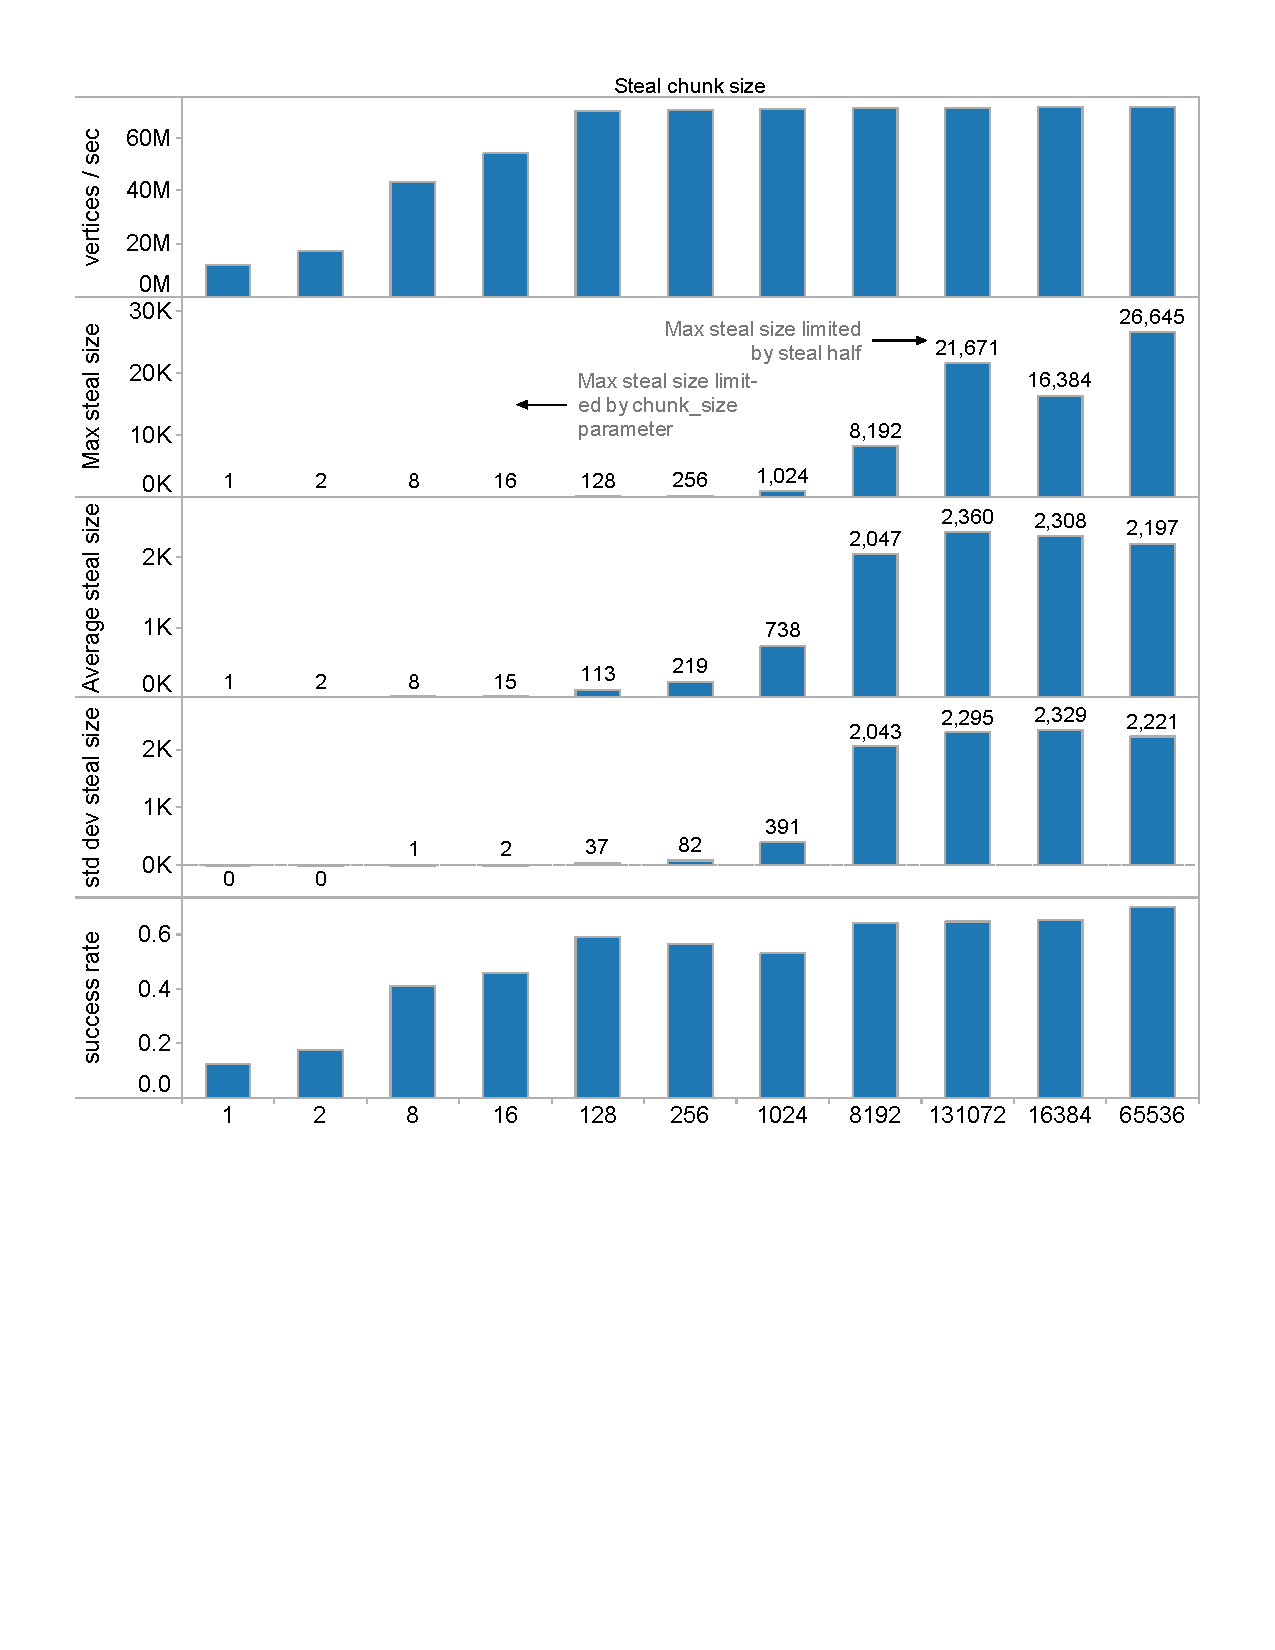
\includegraphics[width=0.5\textwidth]{figs/uts_chunksize.pdf}
%    \end{center}
%    \caption{Performance of UTS-Mem with varying maximum chunk size of
%    steals, run with 30 nodes, 6 cores per node, 4000 workers,
%    \checkme{6M flush ticks}}
%    \label{fig:uts_chunksize}
%\end{figure}


%\TODO{(difference with BFS)}



\subsubsection{Parallel loop threshold}

%\begin{figure}[htb]
%\begin{center}
%  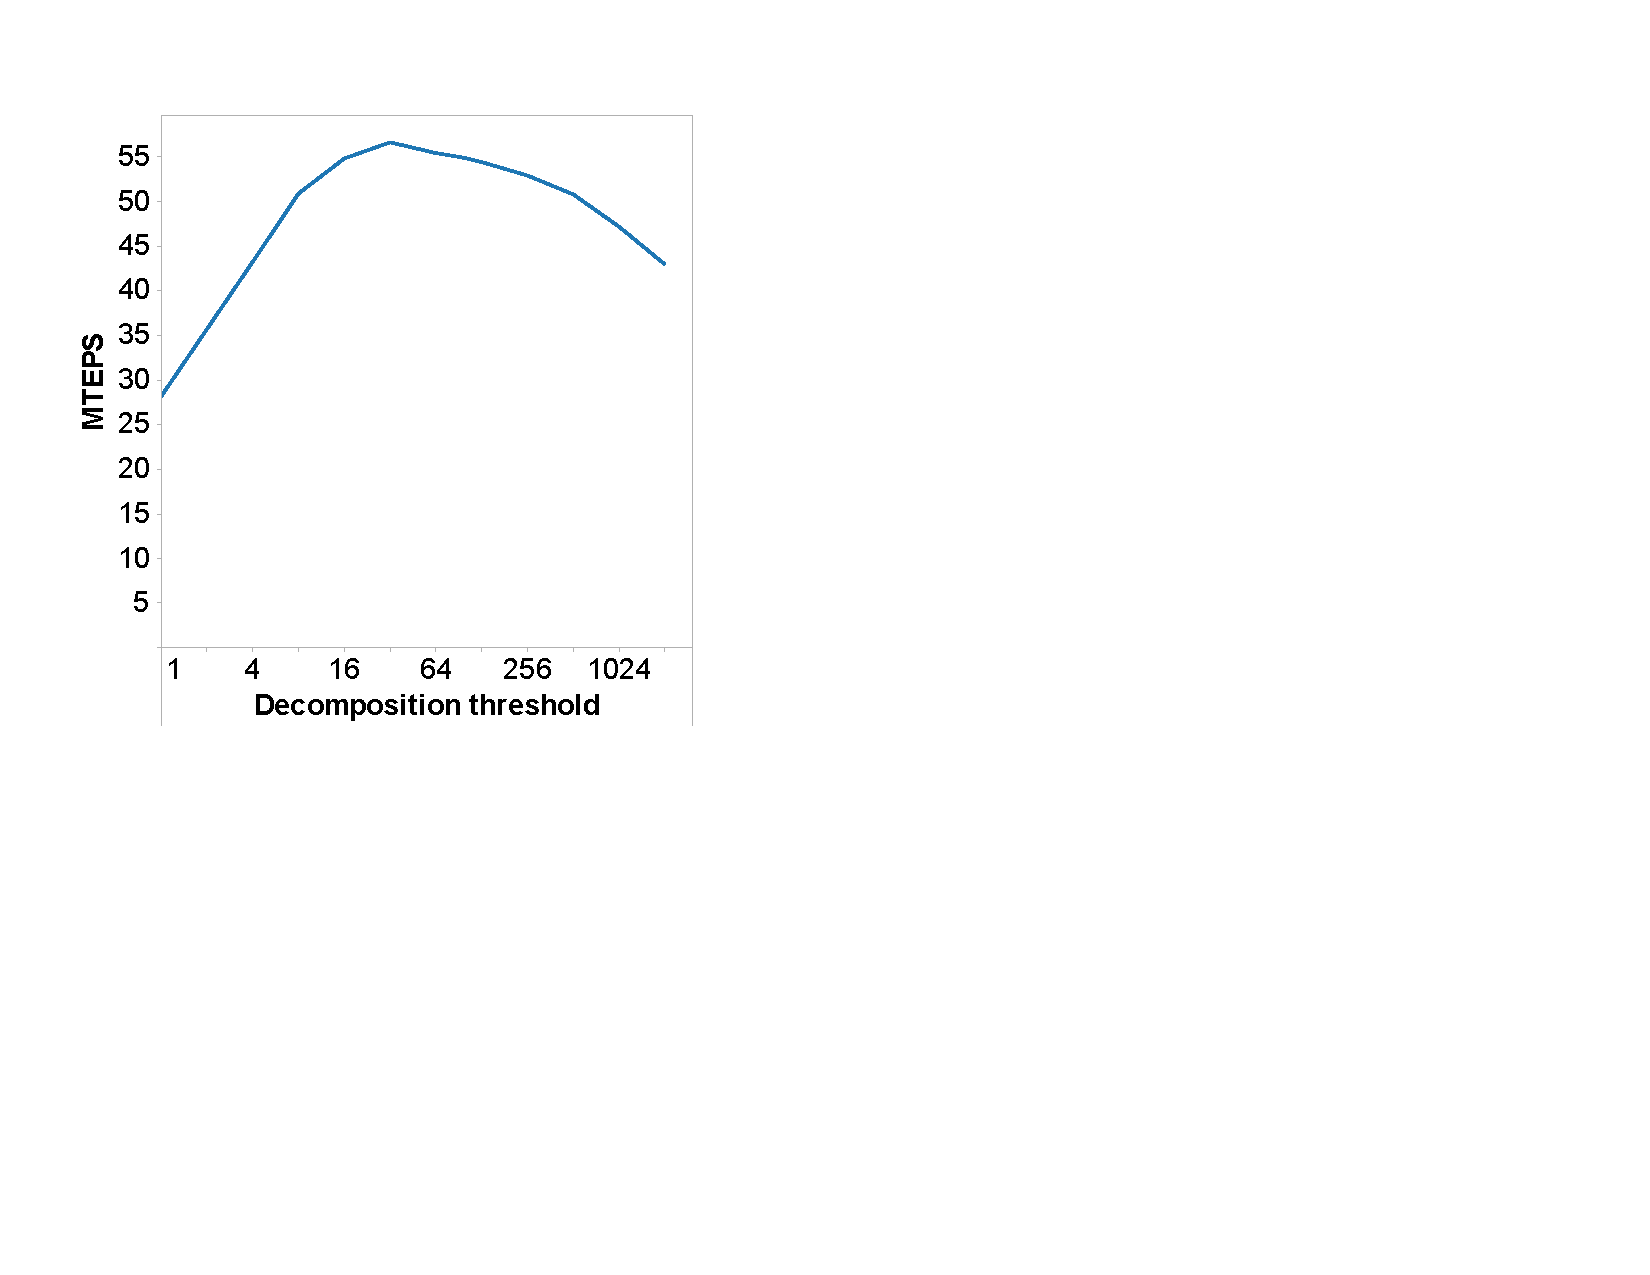
\includegraphics[width=0.95\columnwidth]{figs/bfs_sweep_threshold}
%\begin{minipage}{0.95\columnwidth}
%  \caption{\label{fig:bfs-sweep-threshold} Sensitivity to parallel loop threshold. Note the log scale.}
%\end{minipage}
%\vspace{-3ex}
%\end{center}
%\end{figure}

Parallel overhead---in the form of context switches, task spawns, and
synchronization---can reduce the performance benefit of parallelism.
\Grappa sees a benefit to limiting the amount of parallelism created by
a recursive loop decomposition. The parallel loop threshold (``parallel
granularity'') parameter tells the runtime when to stop creating new tasks and just execute iterations
sequentially. This allows us to amortize the overhead of task
creation. In addition, assigning sequential iterations to a single
task provides the potential to exploit locality when data for adjacent iterations is
also adjacent in memory. The ability to exploit this locality that
exists in the application is an important advantage. We found that in UTS and BFS, increasing the
threshold from 1 up to 8 or 16, respectively, increases performance by
more than 60\%.


% uts threshold
%\begin{figure}[ht]
%    \begin{center}
%      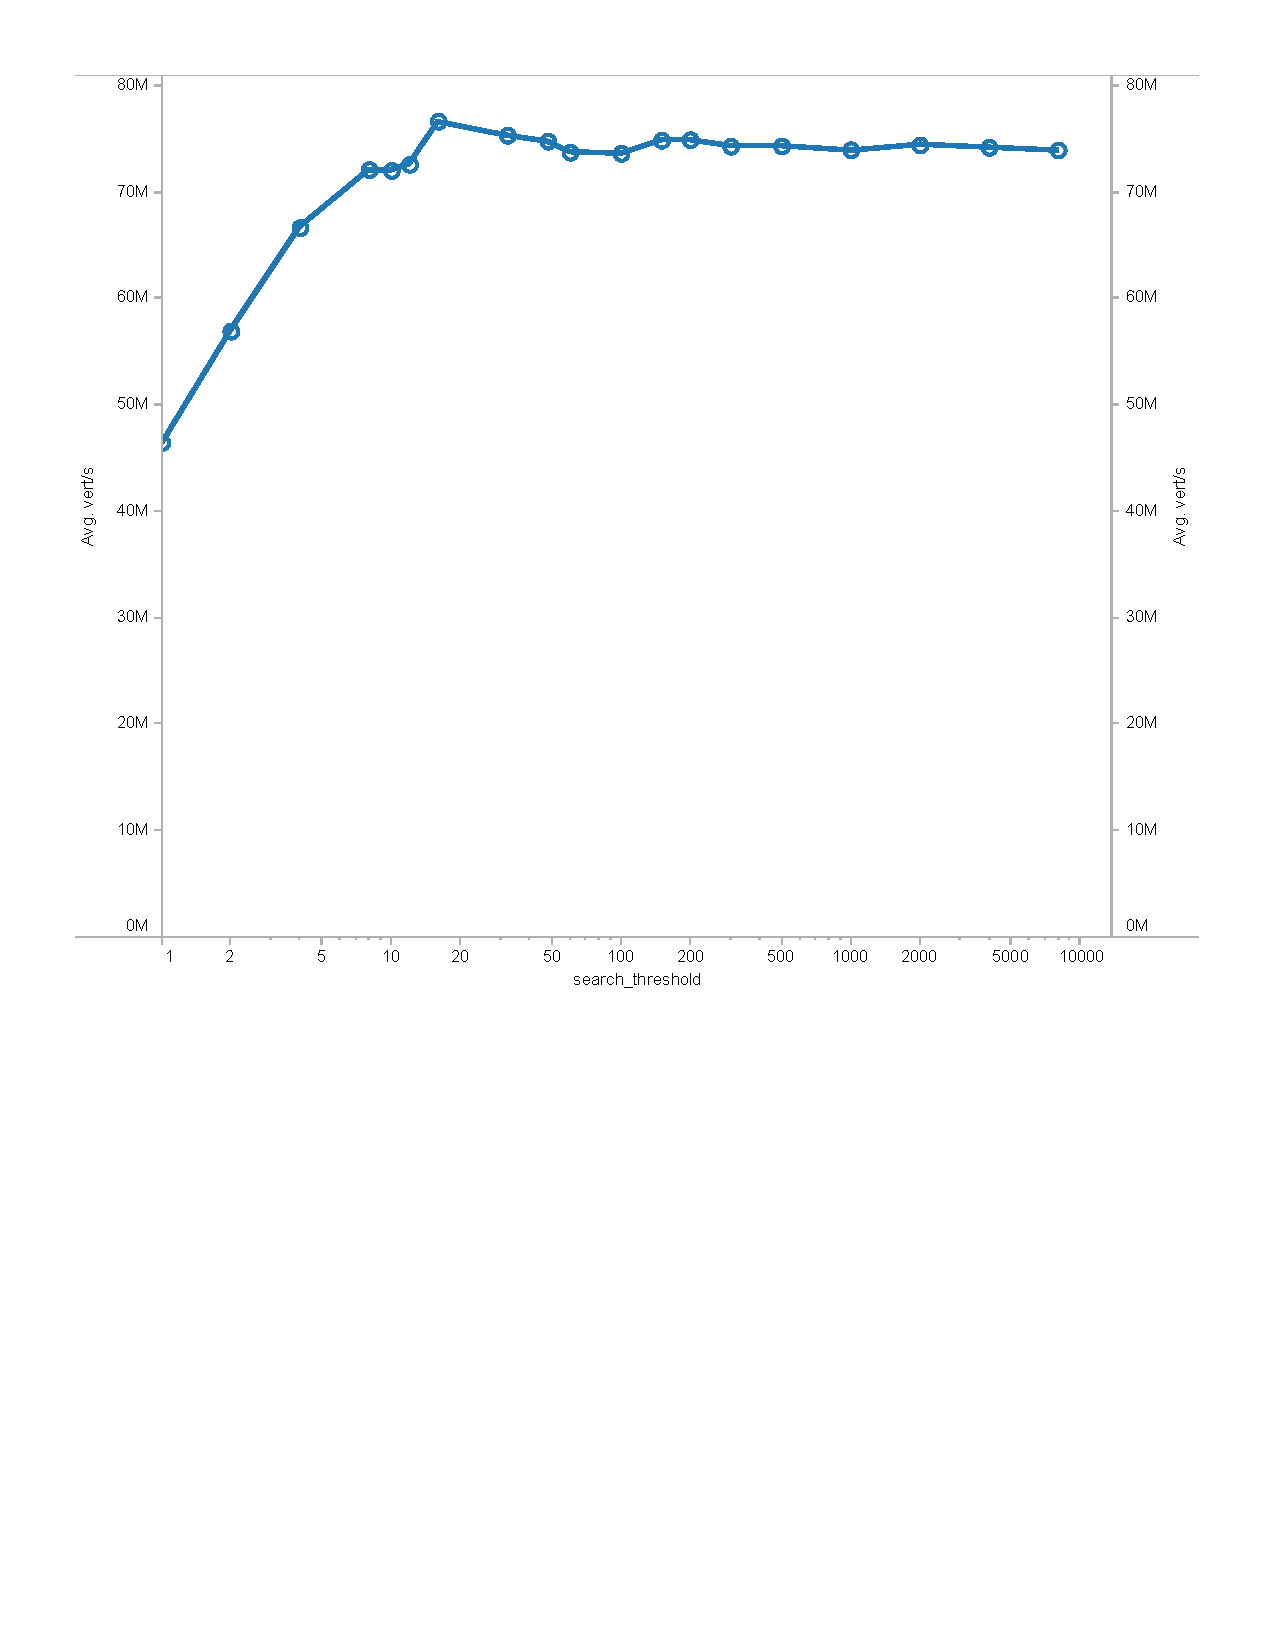
\includegraphics[width=0.5\textwidth]{figs/uts_threshold.pdf}
%    \end{center}
%    \caption{Performance of UTS-Mem with varying parallel loop
%        threshold, run with 30 nodes, 6 cores per node, 4000 workers,
%    \checkme{6M flush ticks}}
%    \label{fig:uts_threshold}
%\end{figure}

\subsection{Summary}\TODO{this is a placeholder: do we need this section?}

\paragraph{Context-switch overhead.} Should we also compare with other packages? (Maybe Capriccio, QThreads?, or even real OS threads?)

\paragraph{Latency.} Measure remote data access latency with and without aggregation turned on.

\paragraph{Aggregated message sizes.} Characterization of the resulting message sizes with aggregation. Right now we only have message size vs. bandwidth.

\paragraph{Utilization.} CPU utilization, Memory, Network. It would be great to answer the question of where is our bottleneck right now. Amount of concurrency with and without aggregation. 

\paragraph{Memory accesses.} Rate of accesses to remote data. Rate of delegate ops. Show limit with GUPs.



%Retries are performed by the memory controller when remote synchronization operations fail to find the full-bit associated with each memory location in the unavailable state.  Retries are issued at low priority relative to new memory operations issued by the processor by other contexts, so they consume what would otherwise be unused injection bandwidth.  On a full-bandwidth system such as the MTA-2, retries have no impact on the progress of tasks other than their own.  On a Cray XMT, network bandwidth is limited, so retries create congestion.  In comparison, \Grappa performs synchronization without retries, delaying responses at the receiving end until ready to notify the sender to proceed.  This saves bandwidth and permits scaling of tasks performing synchronization even on low injection rate networks.


%\begin{figure*}[ht]
%    \begin{minipage}{0.3\linewidth}
%        \centering
%        \includegraphics[width=\textwidth]{figs/chunksize-uts.pdf}
%        \caption{chunksize caption}
%        \label{fig:chunksize-uts}
%    \end{minipage}
%    \begin{minipage}{0.3\linewidth}
%        \centering
%        \includegraphics[width=\textwidth]{figs/workers-uts.pdf}
%        \caption{workers caption}
%        \label{fig:workers-uts}
%    \end{minipage}
%    \begin{minipage}{0.3\linewidth}
%        \centering
%        \includegraphics[width=\textwidth]{figs/thresh-uts.pdf}
%        \caption{threshold caption}
%        \label{fig:thresh-uts}
%    \end{minipage}
%\end{figure*}

}


\section{Related work}

Ways to organize this:
Approaches to graphs: special purpose XMT -> cluster -> distributed frameworks {pregel,graphlab} -> limited programming model -> grappa gen purpose



\subsection{Multithreading to tolerate latency}
Using multithreading to tolerate memory latency is well-covered in the literature. Hardware implementations include the Tera MTA \cite{Tera}, Cray XMT \cite{}, Simultaneous multithreading \cite{}, MIT Alewife \cite{}, Cyclops \cite{}, and even GPUs \cite{fatahalian}.

software threads
lightweight threading

RAMCloud takes a different approach and argues for optimizing networked systems for very low latency with the motivation of getting good performance regardless of access pattern, as well as reducing latency of recovery to reduce backup storage costs.


\subsection{Distribute Shared Memory}

Grappa includes a software distributed shared memory (SDSM). Many traditional SDSM systems are page based [Treadmarks,...], and a lot of work deals with maintaining consistency of data efficiently and optimizing for sharing. Grappa's shared memory is implemented by Active Messages and there is no caching under the hood. Every piece of memory in the shared address space belongs to a single core, and data can be accessed incoherently at any granularity. Grappa provides an API for explicit incoherent caching to take advantage of locality where it exists, as well as sharing. 

Shared memory systems often try to reduce the cost of memory access by predicting good prefetches to overlap memory access and computation; however, this is less effective for irregular applications with fine-grained, data-dependent memory accesses. Grappa depends on high amounts of concurrency to tolerate latency with multithreading.

SDSM systems are usually built to be programmed with flat shared memory programming models like OpenMP, rather than models that make locality explicit like PGAS. 


GASNet is a networking library for supporting portable implmentations of global address space applications or languages, like UPC and recently Chapel...
Grappa currently uses GASNet for networking, but does not use gasnet's mapped shared memory segments for supporting RDMA. Rather, the global address space is implemented at a higher level using Active Messages.

RAMCloud - RPC call communication abstraction like us because it supports more flexibility,...


Difference from txDSM \cite{sdsm-with-txn-coherence} is that we don't try to provide txns over multiple nodes, only within one core's memory.

\subsection{Partitioned Global Address space}
The goal of presenting a global view of distributed memory to the programmer is shared by the PGAS community, and is used in languages like Chapel \cite{Chapel}, X10 \cite{X10}, and UPC \cite{UPC}. In these programming models, access to shared structures look like normal memory references, but the programmer tries to minimize references to remote nodes. Unlike the usual programming goal in PGAS, since we target problems with poor locality, we design Grappa for remote references as a common case. Thread private data is still local, and unlike the XMT, we exploit locality where it does exist in an application (such as spatial locality in a graph edgelist), but we design the system to perform well in the midst of mostly remote accesses to large shared data structures. We would like to implement PGAS languages that support dynamic parallelism, like Chapel, in Grappa.

\subsection{Programming models for distributed graph processing}

Distributed graph processing frameworks like Pregel \cite{pregel:2010} and Distributed GraphLab \cite{distgraphlab:vldb12} provide graph-parallel, vertex-centric programming abstractions that free the application writer from solving distributed system issues like scheduling parallelism, handling fault tolerance, and scaling communication. Pregel adopts a bulk-synchronous parallel (BSP) execution model, which makes it inefficient on workloads that could prioritize vertices. GraphLab, on the other hand, schedules vertex computations individually, allowing prioritization, which gives faster convergence in a variety of iterative algorithms. Grappa also supports dynamic parallelism with asynchronous execution, but has a more general purpose programming model, where parallelism is expressed as tasks or loop iterations. \TODO{and express locality? How much to talk about how graphlab achieves scalable performance?}

\TODO{should we mention GreenMarl and how its first distributed try is compile down to Pregel}


\section{Conclusion}

Irregular computations are both important and challenging to execute
quickly.  Scaling these applications easily on commodity hardware has
been a historical challenge. \Grappa is a runtime framework that
simplifies this task for software developers and compiler
writers. This paper describes the \Grappa framework and its three main
components: a task library, a distributed shared memory system, and a
network aggregator. \Grappa's key aspect is extreme latency tolerance,
which not only hides network latency but also enables the system to
spend time on sophisticated work stealing and network optimizations,
trading latency for even more throughput.

Our evaluation of \Grappa reveals that the core components, scheduling
and communication, achieve their design goals.  Thousands of workers
can be efficiently context switched on a multicore processor, up to
the DRAM bandwidth.  Aggregating messages enables \Grappa to achieve
over 1.0~GUPS on 64~nodes.  We also explored four other algorithms:
unbalanced tree search, breadth first search, PageRank, and integer
sort, comparing performance of these algorithms on \Grappa, the Cray
XMT, and optimized MPI implementations.

Depending on the benchmark, \Grappa is between 11X faster and 5.4X
slower than MPI and UPC, and between 2.6X faster and 4.3X slower than
the XMT. When \Grappa is slower than MPI, we find that the MPI
implementation includes a specialized implementation of a feature
\Grappa provides generally to all applications. This generality comes
at a performance cost but eases the application developer's
task. Moreover, significant tuning has yet to be done on the \Grappa
runtime system.  Yet when cost-performance is considered, mass-market
x86-based cluster hardware makes \Grappa a highly attractive option.


%
\section{Acknowledgements}

A portion of this work was performed using PNNL Institutional
Computing at Pacific Northwest National Laboratory; we thank Tim
Carlson for his help in configuring the cluster. We thank the HPC
Advisory Council for the use of their clusters.


%\subsection{References}
\bibliographystyle{abbrv}
\bibliography{paper,generals}

\end{document}

